\documentclass[aspectratio=169]{beamer}
\mode<presentation>
\usetheme{Madrid}
\usecolortheme{seahorse}
% \usepackage[table]{xcolor}
\usepackage{multimedia}
\usepackage{media9}
\usepackage[utf8]{inputenc}
\usepackage{amsmath}
\usepackage{lmodern}
% \usepackage[usenames, dvipsnames]{color}
\usepackage{threeparttable}

\usepackage{arydshln}
\usepackage{url}
\usepackage[absolute,overlay]{textpos}
% \usepackage[texcoord,grid,gridunit=cm,gridcolor=red!50,subgridcolor=green!50]{eso-pic}
\setlength{\TPHorizModule}{\textwidth}
\setlength{\TPVertModule}{\textwidth}

\graphicspath{{plots/}}

\setbeamercolor{CBwonb}{fg=white,bg=white!10!blue}
\setbeamercolor{CBronb}{fg=red,bg=white!10!blue}

\usepackage{tikz}
\usetikzlibrary{shapes,arrows,positioning}
\tikzstyle{startstop} = [rectangle, rounded corners, minimum width=1cm, minimum height=0.1cm,text centered, text width=2.5cm, draw=black, fill=red!30]
\tikzstyle{io} = [trapezium, trapezium left angle=70, trapezium right angle=110, minimum width=1cm, minimum height=0.1cm, text centered, text width=2.5cm, draw=black, fill=blue!30]
\tikzstyle{process} = [rectangle, minimum width=1cm, minimum height=0.1cm, text centered,text width=2.5cm, draw=black, fill=orange!30]
\tikzstyle{decision} = [circle, minimum width=1cm, minimum height=0.1cm, text centered,text width=2.5cm, draw=black, fill=green!30]
\tikzstyle{arrow} = [thick,->,text centered, color=blue, text width=2cm,>=stealth]

\newcommand{\Msun}{~{\rm M_\sun}}
\newcommand{\hMsun}{~h^{-1}\>{\rm M_\odot}}
\newcommand{\Mpc}{~h^{-1}~{\rm Mpc}}
\newcommand{\Kpc}{~h^{-1}~{\rm kpc}}


\title[]{The Large-Scale Environments}
\subtitle{The large-scale distribution of baryons inside the cosmological
hydrodynamical simualtions.}
\author[]{{\Large \bf Weiguang Cui},
\inst{*} \footnote{Email: wcui@roe.ac.uk; ~ ~ Homepage: \url{https://weiguangcui.github.io}}}
\institute[]{
  \inst{*}
    Institute for Astronomy, University of Edinburgh, Royal Observatory of Edinburgh,\\
    Edinburgh EH9 3HJ, United Kingdom
}
\date[]{NAM, @Lancaster \\  July, 01, 2019}


%%%%%%%%%%%%%%%%%%%%%%%%%%%%%%%%%%%%%%%%%%%%%%%%%%%%%%%%%%%%%%%%%%%%%%%%%
\begin{document}
  \frame{\titlepage}

\begin{frame}[plain,c]
    \begin{figure}
        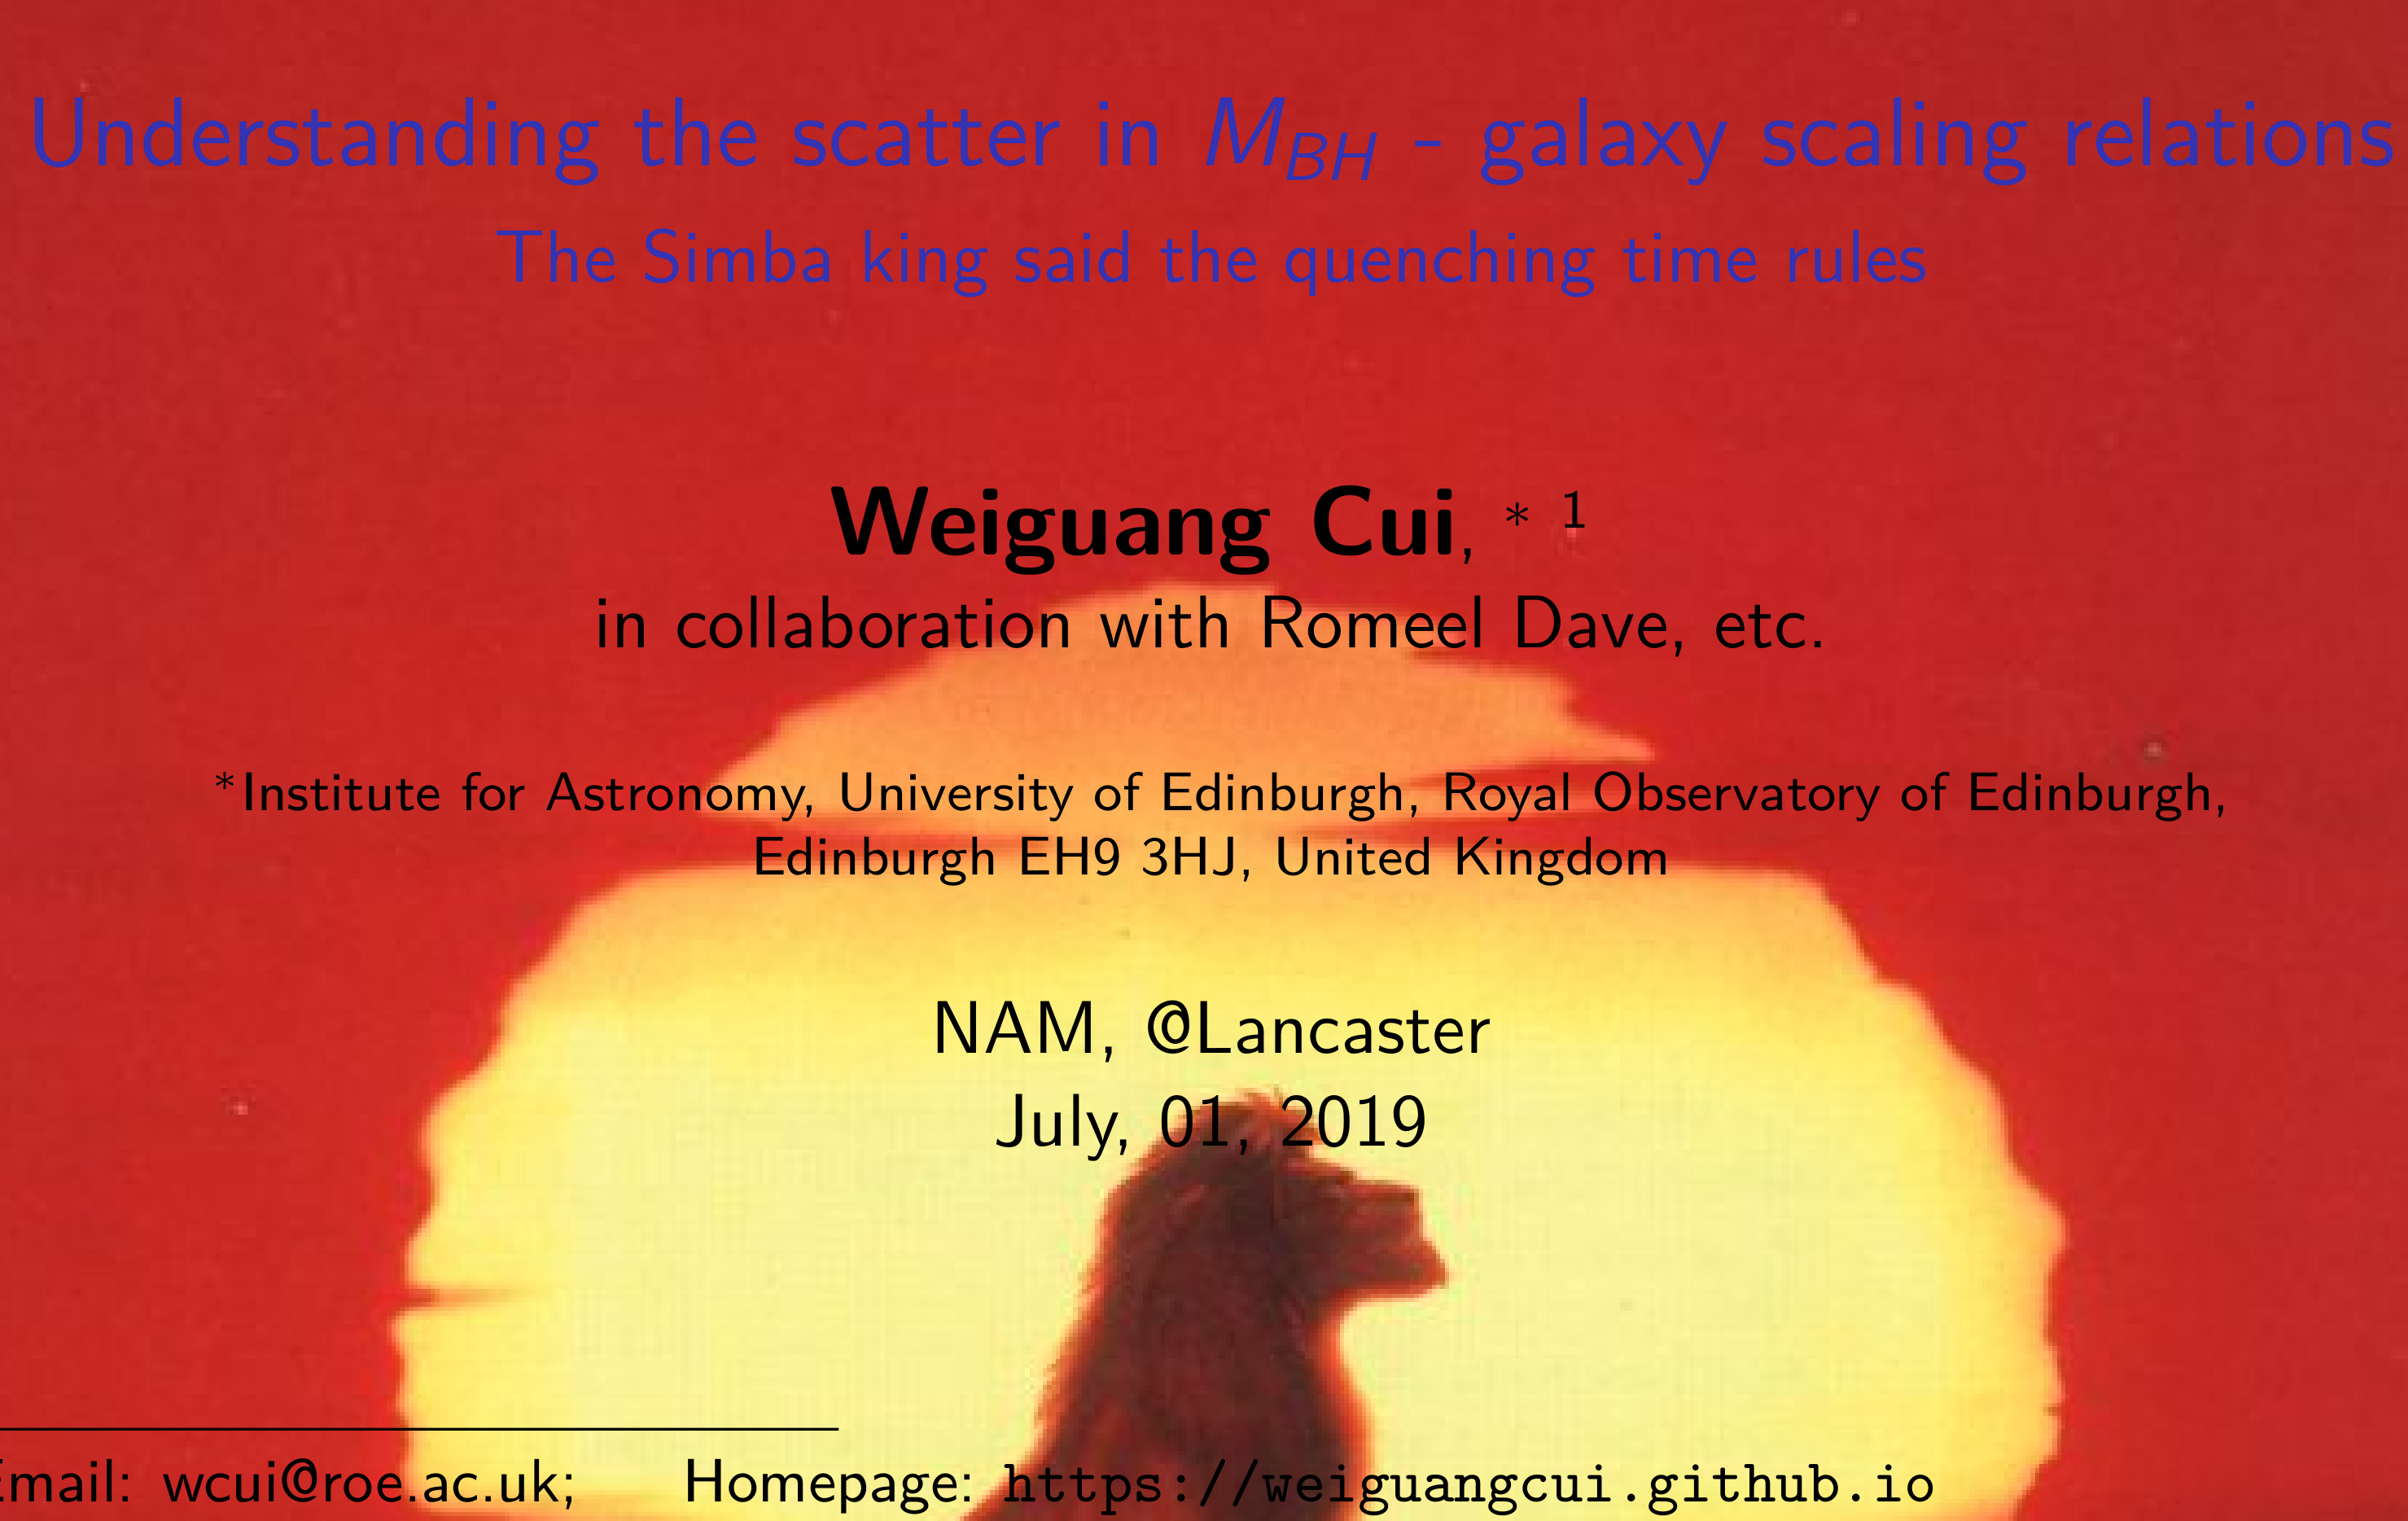
\includegraphics[width=0.488\textwidth]{talk-simba.png}
        \includegraphics[width=0.512\textwidth]{talk-300.png}
    \end{figure}
\end{frame}

%----------------------------------
\section{Introduction} \label{sec:1}

\begin{frame}[plain,t]
    \begin{textblock*}{4cm}(0.5cm,.6cm)
        {The content of the Universe:}
    \end{textblock*}
    \begin{figure}
        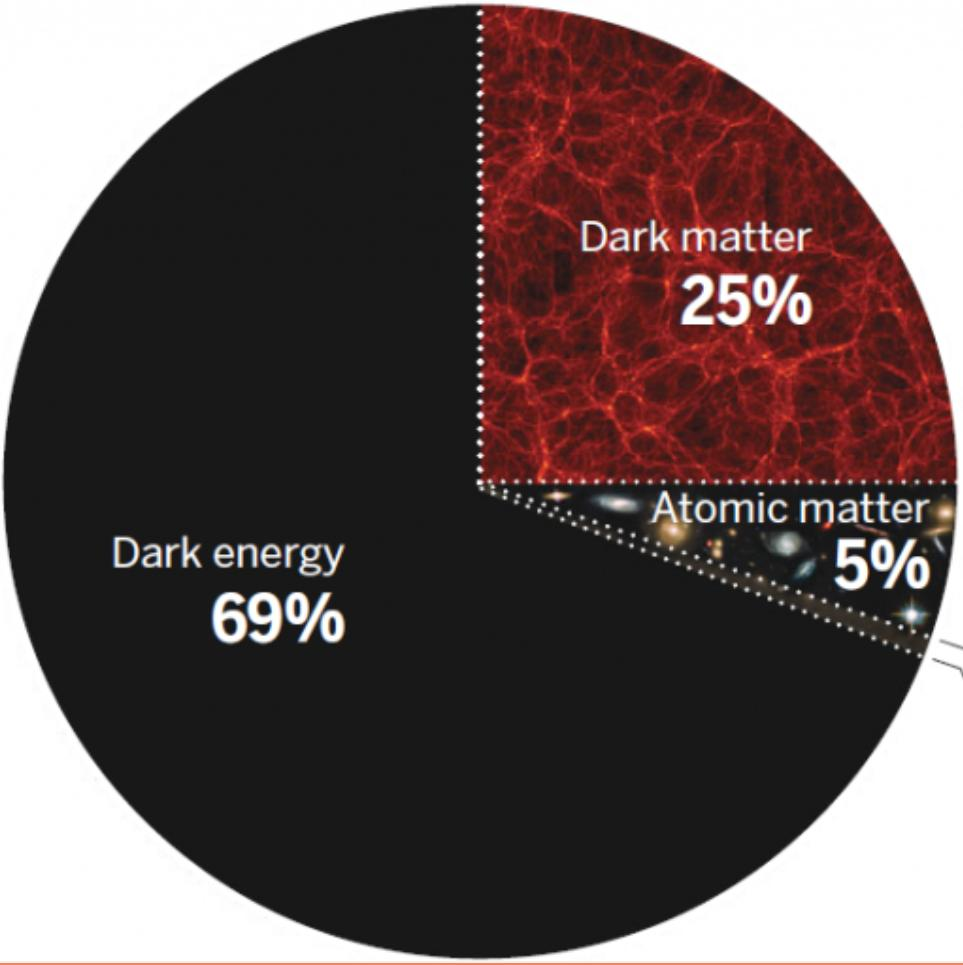
\includegraphics[height=\textheight]{fraction.jpg}
    \end{figure}
    \begin{textblock*}{3cm}(12.5cm,6.cm)
        {$\sim$1\% of neutrinos, etc.}
    \end{textblock*}
\end{frame}

\begin{frame}[plain,t]
    \begin{textblock*}{4cm}(0.5cm,.6cm)
        {The content of the baryons:}
    \end{textblock*}
    \begin{figure}
        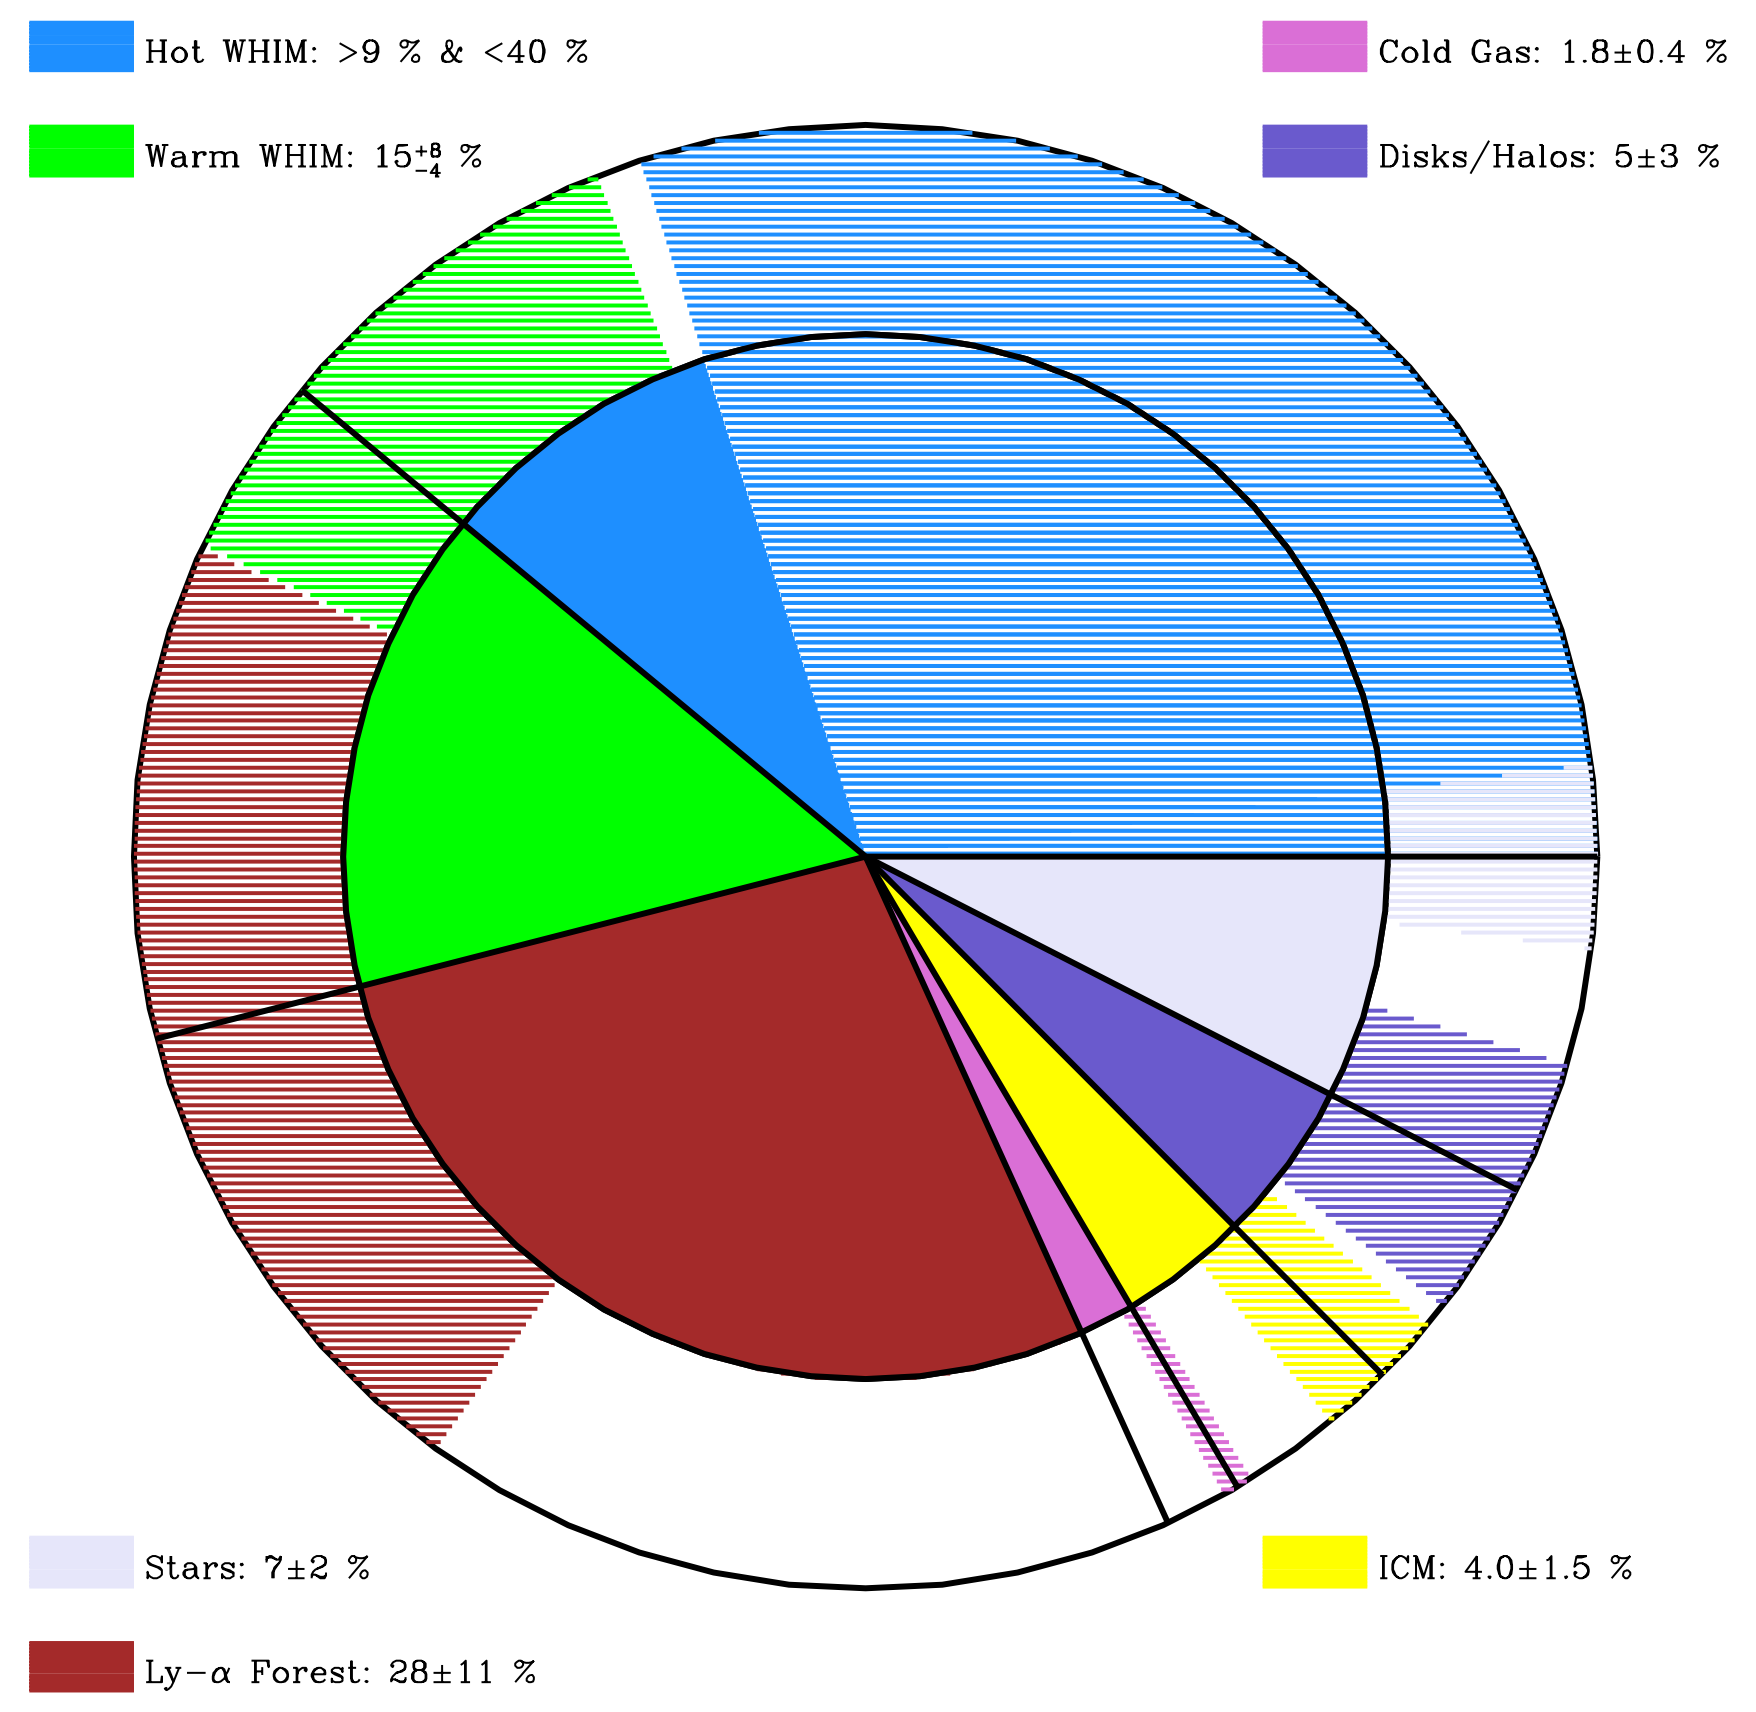
\includegraphics[height=\textheight]{baryon-fraction.png}
    \end{figure}
    \begin{textblock*}{3cm}(12.5cm,6.cm)
        {Nicastro et al. 2018}
    \end{textblock*}
\end{frame}

\begin{frame}[plain,t]
%   \frametitle{Background: the distribution of dark matter at large scale}
%   \framezoom<1><2>[](5cm,3.5cm)(1.5cm,1.5cm)
  \begin{figure}
    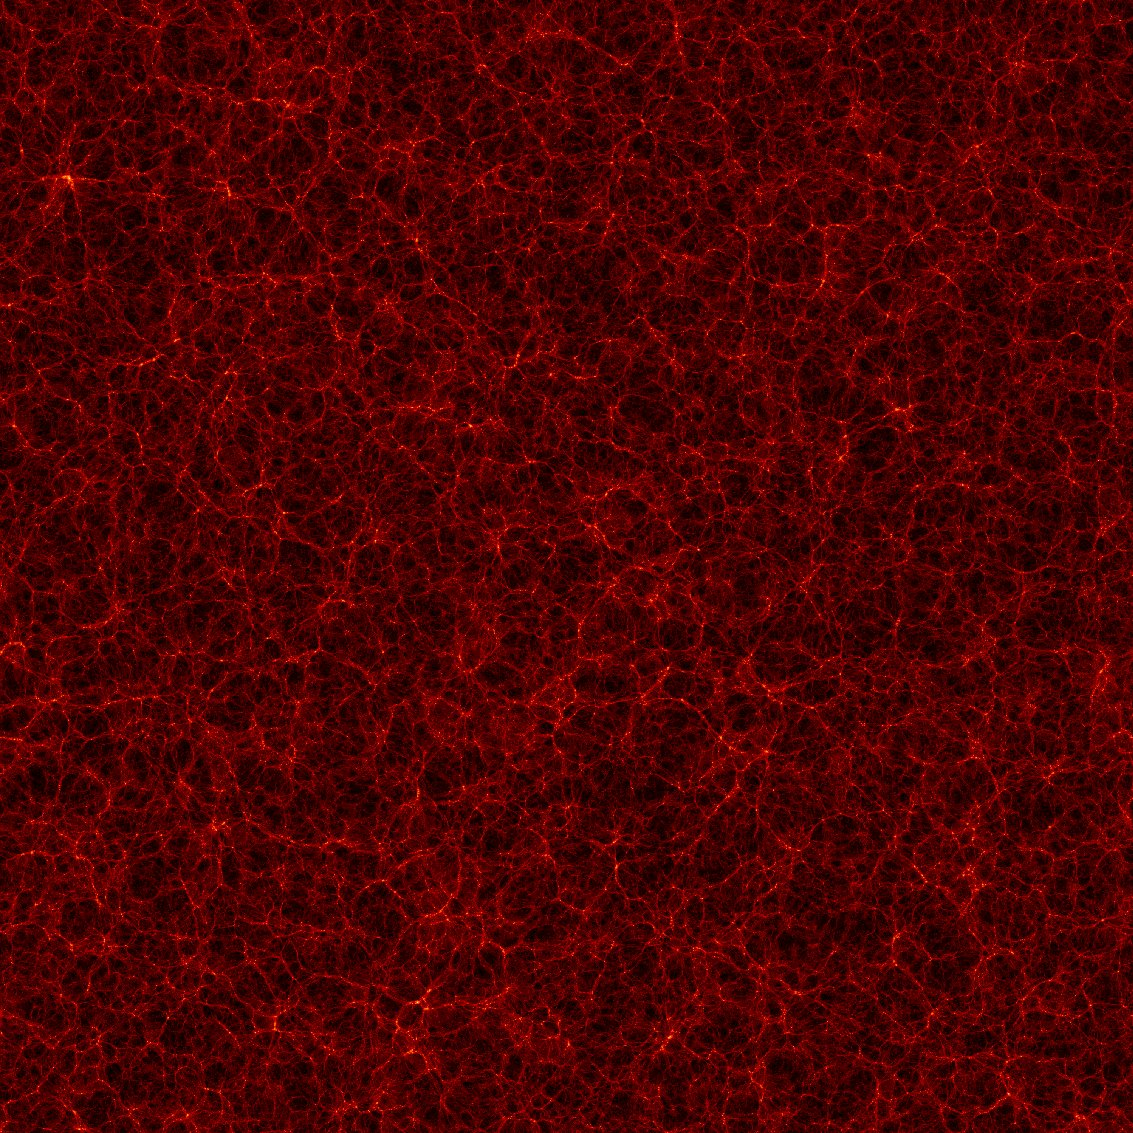
\includegraphics[height=0.65\textheight]{mdpl.jpg} ~ 
    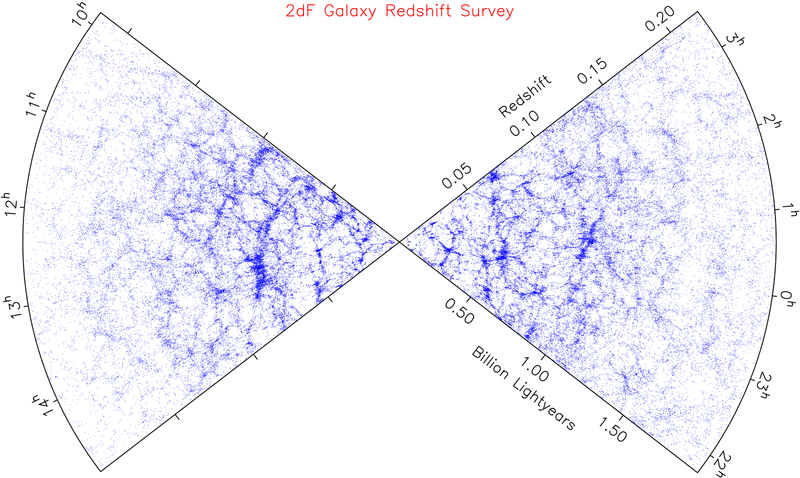
\includegraphics[height=0.65\textheight]{2dFzcone.jpg}
  \end{figure}
  \begin{textblock*}{6cm}(0.5cm,7.5cm)
    {Credit: MultiDark Planck simulation}
  \end{textblock*}
    \begin{textblock*}{4cm}(9cm,7.5cm)
    {Credit: Yang et al. 2005}
  \end{textblock*}
\end{frame}

\begin{frame}[plain,c]
    \begin{center}
        \Huge{Where are the gas?}
        % \par
    \end{center}
\end{frame}

\begin{frame}[plain,t]
    \only<1->{
     \begin{textblock*}{7cm}(0.3cm,0.cm)
     \vspace{-0.2cm}
        \begin{figure}
         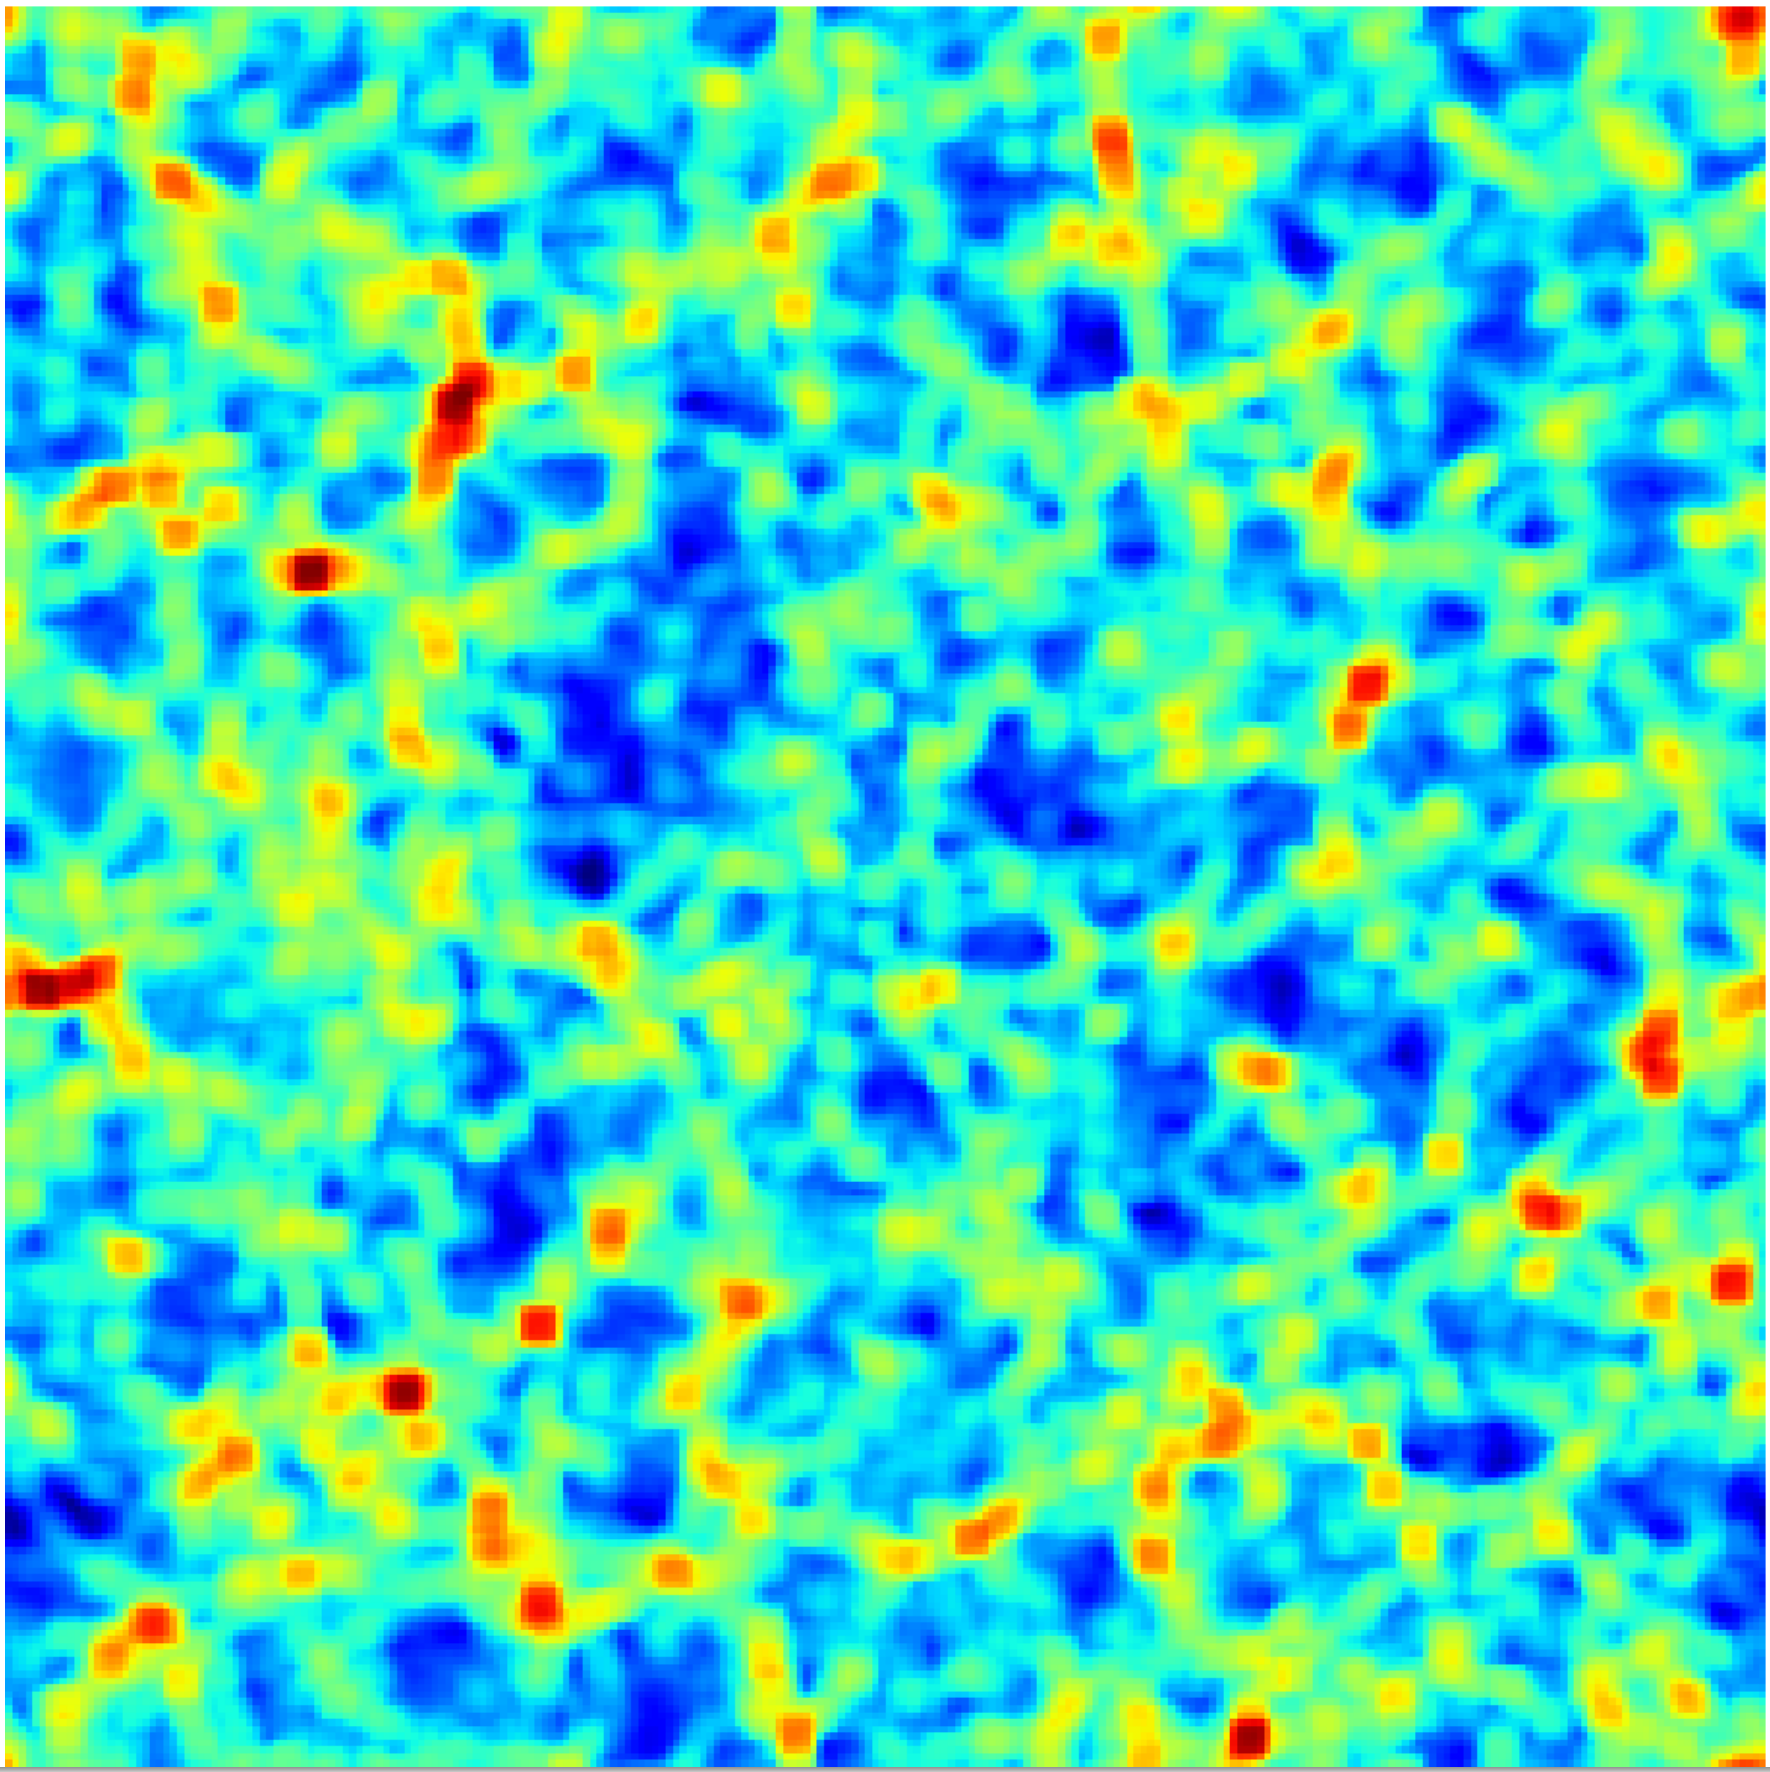
\includegraphics[height=0.88\textheight]{gas-density.png}
         \caption{Gas density, Cui et al. 2019}
        \end{figure}
    \end{textblock*} 
  }
  \only<2->{
  \begin{textblock*}{7cm}(8.3cm,0.cm)
  \vspace{-0.2cm}
    \begin{figure}
    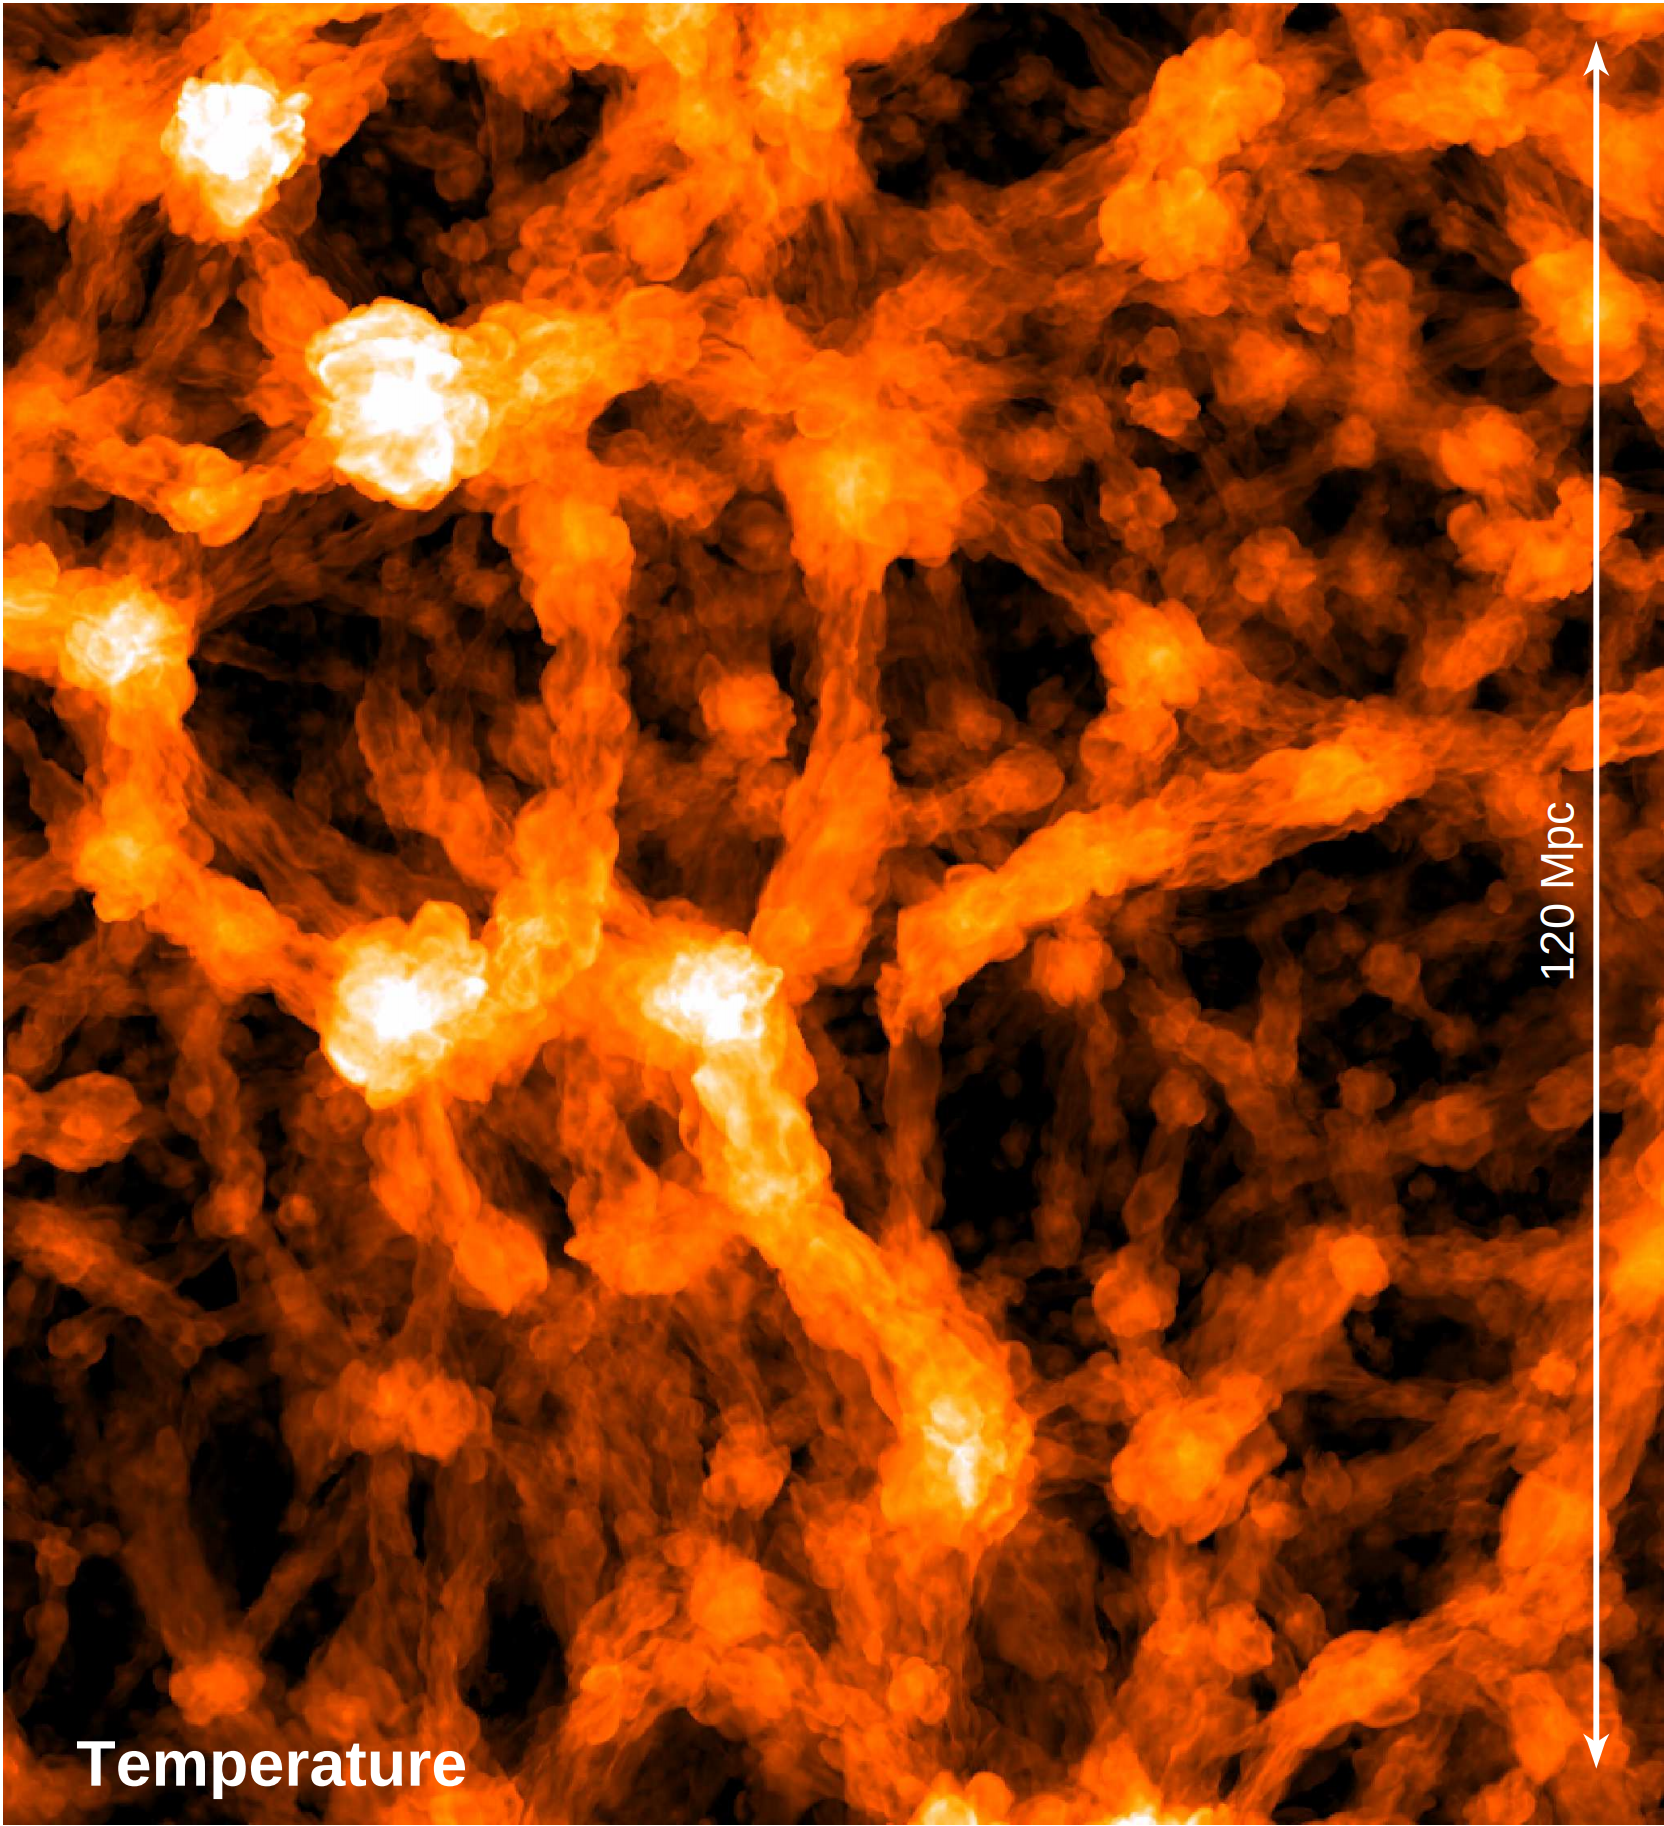
\includegraphics[height=0.88\textheight]{gas-temperature.png}
    \caption{Gas temperature, Vazza et al. 2015}
  \end{figure}
    \end{textblock*}  
    }
  \only<3->{
    \begin{textblock*}{15cm}(.3cm,0.cm)
    \vspace{-0.3cm}
     \begin{figure}
    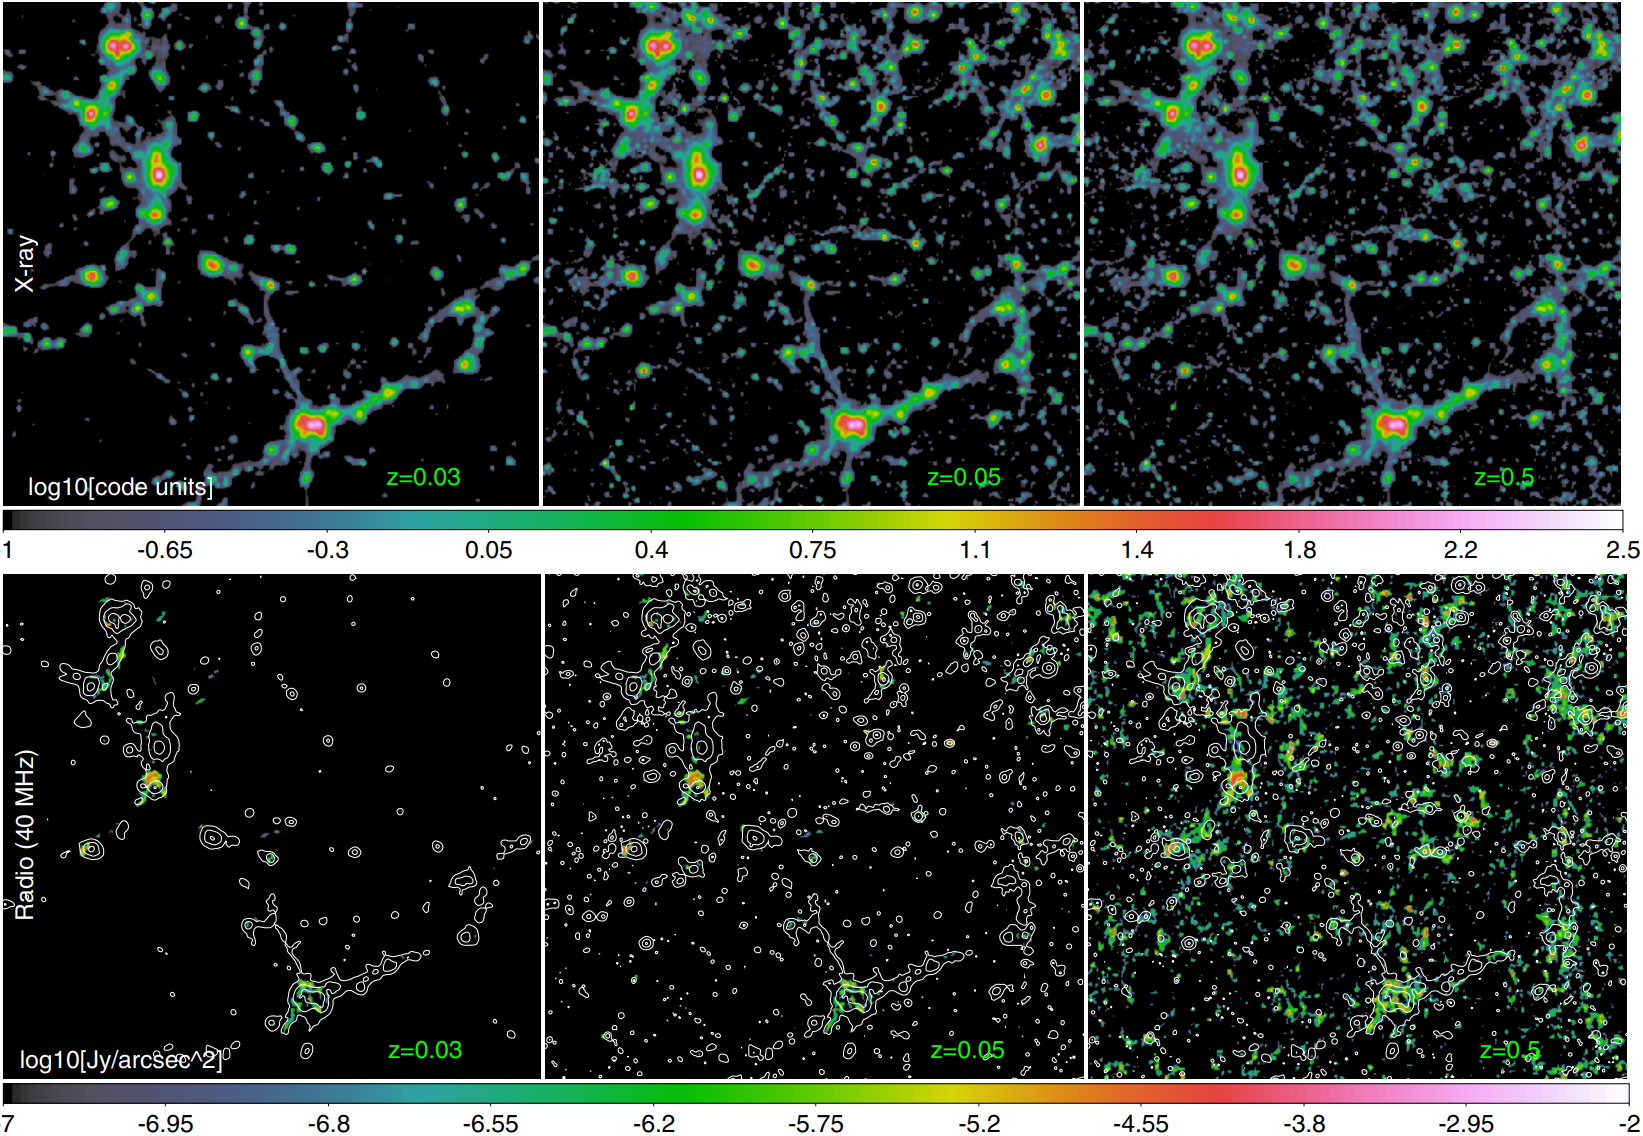
\includegraphics[height=\textheight]{xray-radio-web.png}
    \vspace{-0.5cm}
    \caption{Mock X-ray and radio image, Vazza et al. 2015}
  \end{figure}
    \end{textblock*}
  }
\end{frame}

\begin{frame}[plain,c]
  \Large{The aim of {\bf The Large-Scale Environments project} is to study the distribution and abundance of baryonic matter at large-scale.}
  
  \bigskip
  
  \begin{itemize}
    \item<2-> The hydro-simulations for this study.
    \item<3-> How to classify the large-scale environments?
    \item<4-> What does the simulation say about the baryon distribution?
    \item<5-> Conclusion and future prospects.
  \end{itemize}
\end{frame}

\section{simulations}
\begin{frame}{The cosmological hydrodynamical simulations}
Three versions of simulations with different sets of baryonic models are used for this study:
\begin{itemize}
    \item RDM -- dark-matter-only simulation; 
    \item CSF -- gas Cooling, Star formation and Supernovae feedback;
    \item AGN -- additional BH evolution and feedback are also included.
\end{itemize}
\vspace{-0.6cm}
\begin{table}
\fontsize{9}{9}\selectfont
\caption{Parameters of the Three Hundred simulations}
\begin{tabular}{lll}
  \hline
  Parameter& Value & Description\\
  \hline
  $\Omega_M$ & 0.24 & Total Matter density parameter\\
  $\Omega_B$ & 0.041 & Baryon density parameter\\
  $\Omega_\Lambda$ & 0.76 & Cosmological Constant density parameter\\
  $h$ & 0.73  & Hubble constant in units of 100 km/s/Mpc\\
  $\sigma_8$ & 0.8 & Normalization of Power spectrum\\
  $n_s$ & 0.96  & Power index\\
  $\epsilon_{phys}$ & 7.5 & Plummer equivalent softening in $\Kpc$ \\
  Box size & \alert{410} & [$\Mpc$] The simulation box size on one side \\
  Particle mass & $7.6 (35.4) $ & [$10^8 \hMsun$] gas (DM) particle mass \\
  \hline
\end{tabular}
\end{table}
Details can be found in Cui et al. 2014.
\end{frame}

\section{The classification methods}
\begin{frame}{The classification methods -- Vweb and Pweb\footnote{{\footnotesize Also called T-web}}}
\only<1->{
\begin{textblock*}{15cm}(0.4cm,1.3cm)
The re-scaled Poisson equation: $\Delta^2 \phi = \delta$ with $\delta$ the dimensionless matter overdensity and $\phi$ is the potential.
\end{textblock*}}
\only<2->{
\begin{textblock*}{15cm}(0.4cm,2.2cm)
\vspace{-1cm}
  \begin{columns}[t]
    \begin{column}{0.49\textwidth}
      \begin{block}{Pweb (Hahn et al. 2005):}
      The tidal tensor, $T_{\alpha\beta}$, is defined by the Hessian of the
gravitational potential $\phi$:
     $T_{\alpha\beta} = \frac{\partial^2\phi}{\partial r_{\alpha} \partial r_{\beta}}.$
      \end{block}
    \end{column}
    \begin{column}{0.49\textwidth}
      \begin{block}{Vweb (Hoffman et al. 2012):}
    The shear tensor, which is rewritten as
    $\Sigma_{\alpha, \beta} = -\frac{1}{2}(\frac{\partial v_{\alpha}}{\partial r_{\beta}} + \frac{\partial v_{\beta}}{\partial r_{\alpha}})/H_0$ 
      \end{block}
    \end{column}
  \end{columns}
\end{textblock*}}
\only<3->{
\begin{textblock*}{15cm}(0.4cm,5.2cm)
 The three eigenvalues $\lambda_1 > \lambda_2 > \lambda_3$ are used to determine the large-scale environments:
 \begin{itemize}
     \item Voids: if $\lambda_1 < \lambda_{th}$
     \item Sheets: if $\lambda_1 >= \lambda_{th} > \lambda_2$
     \item Filaments: if $\lambda_2 >= \lambda_{th} > \lambda_3$
     \item Knots: $\lambda_3 >= \lambda_{th}$
 \end{itemize}
\end{textblock*}
\begin{textblock*}{3cm}(9.5cm,6cm)
{$\lambda_{th} = 0.01$ for Pweb; $\lambda_{th} = 0.1$ for Vweb}
\end{textblock*}}
\end{frame}

\section{Results}
\begin{frame}[plain,t]
\begin{textblock*}{6.5cm}(1.5cm,0.1cm)
\vspace{-0.3cm}
  \begin{figure}
    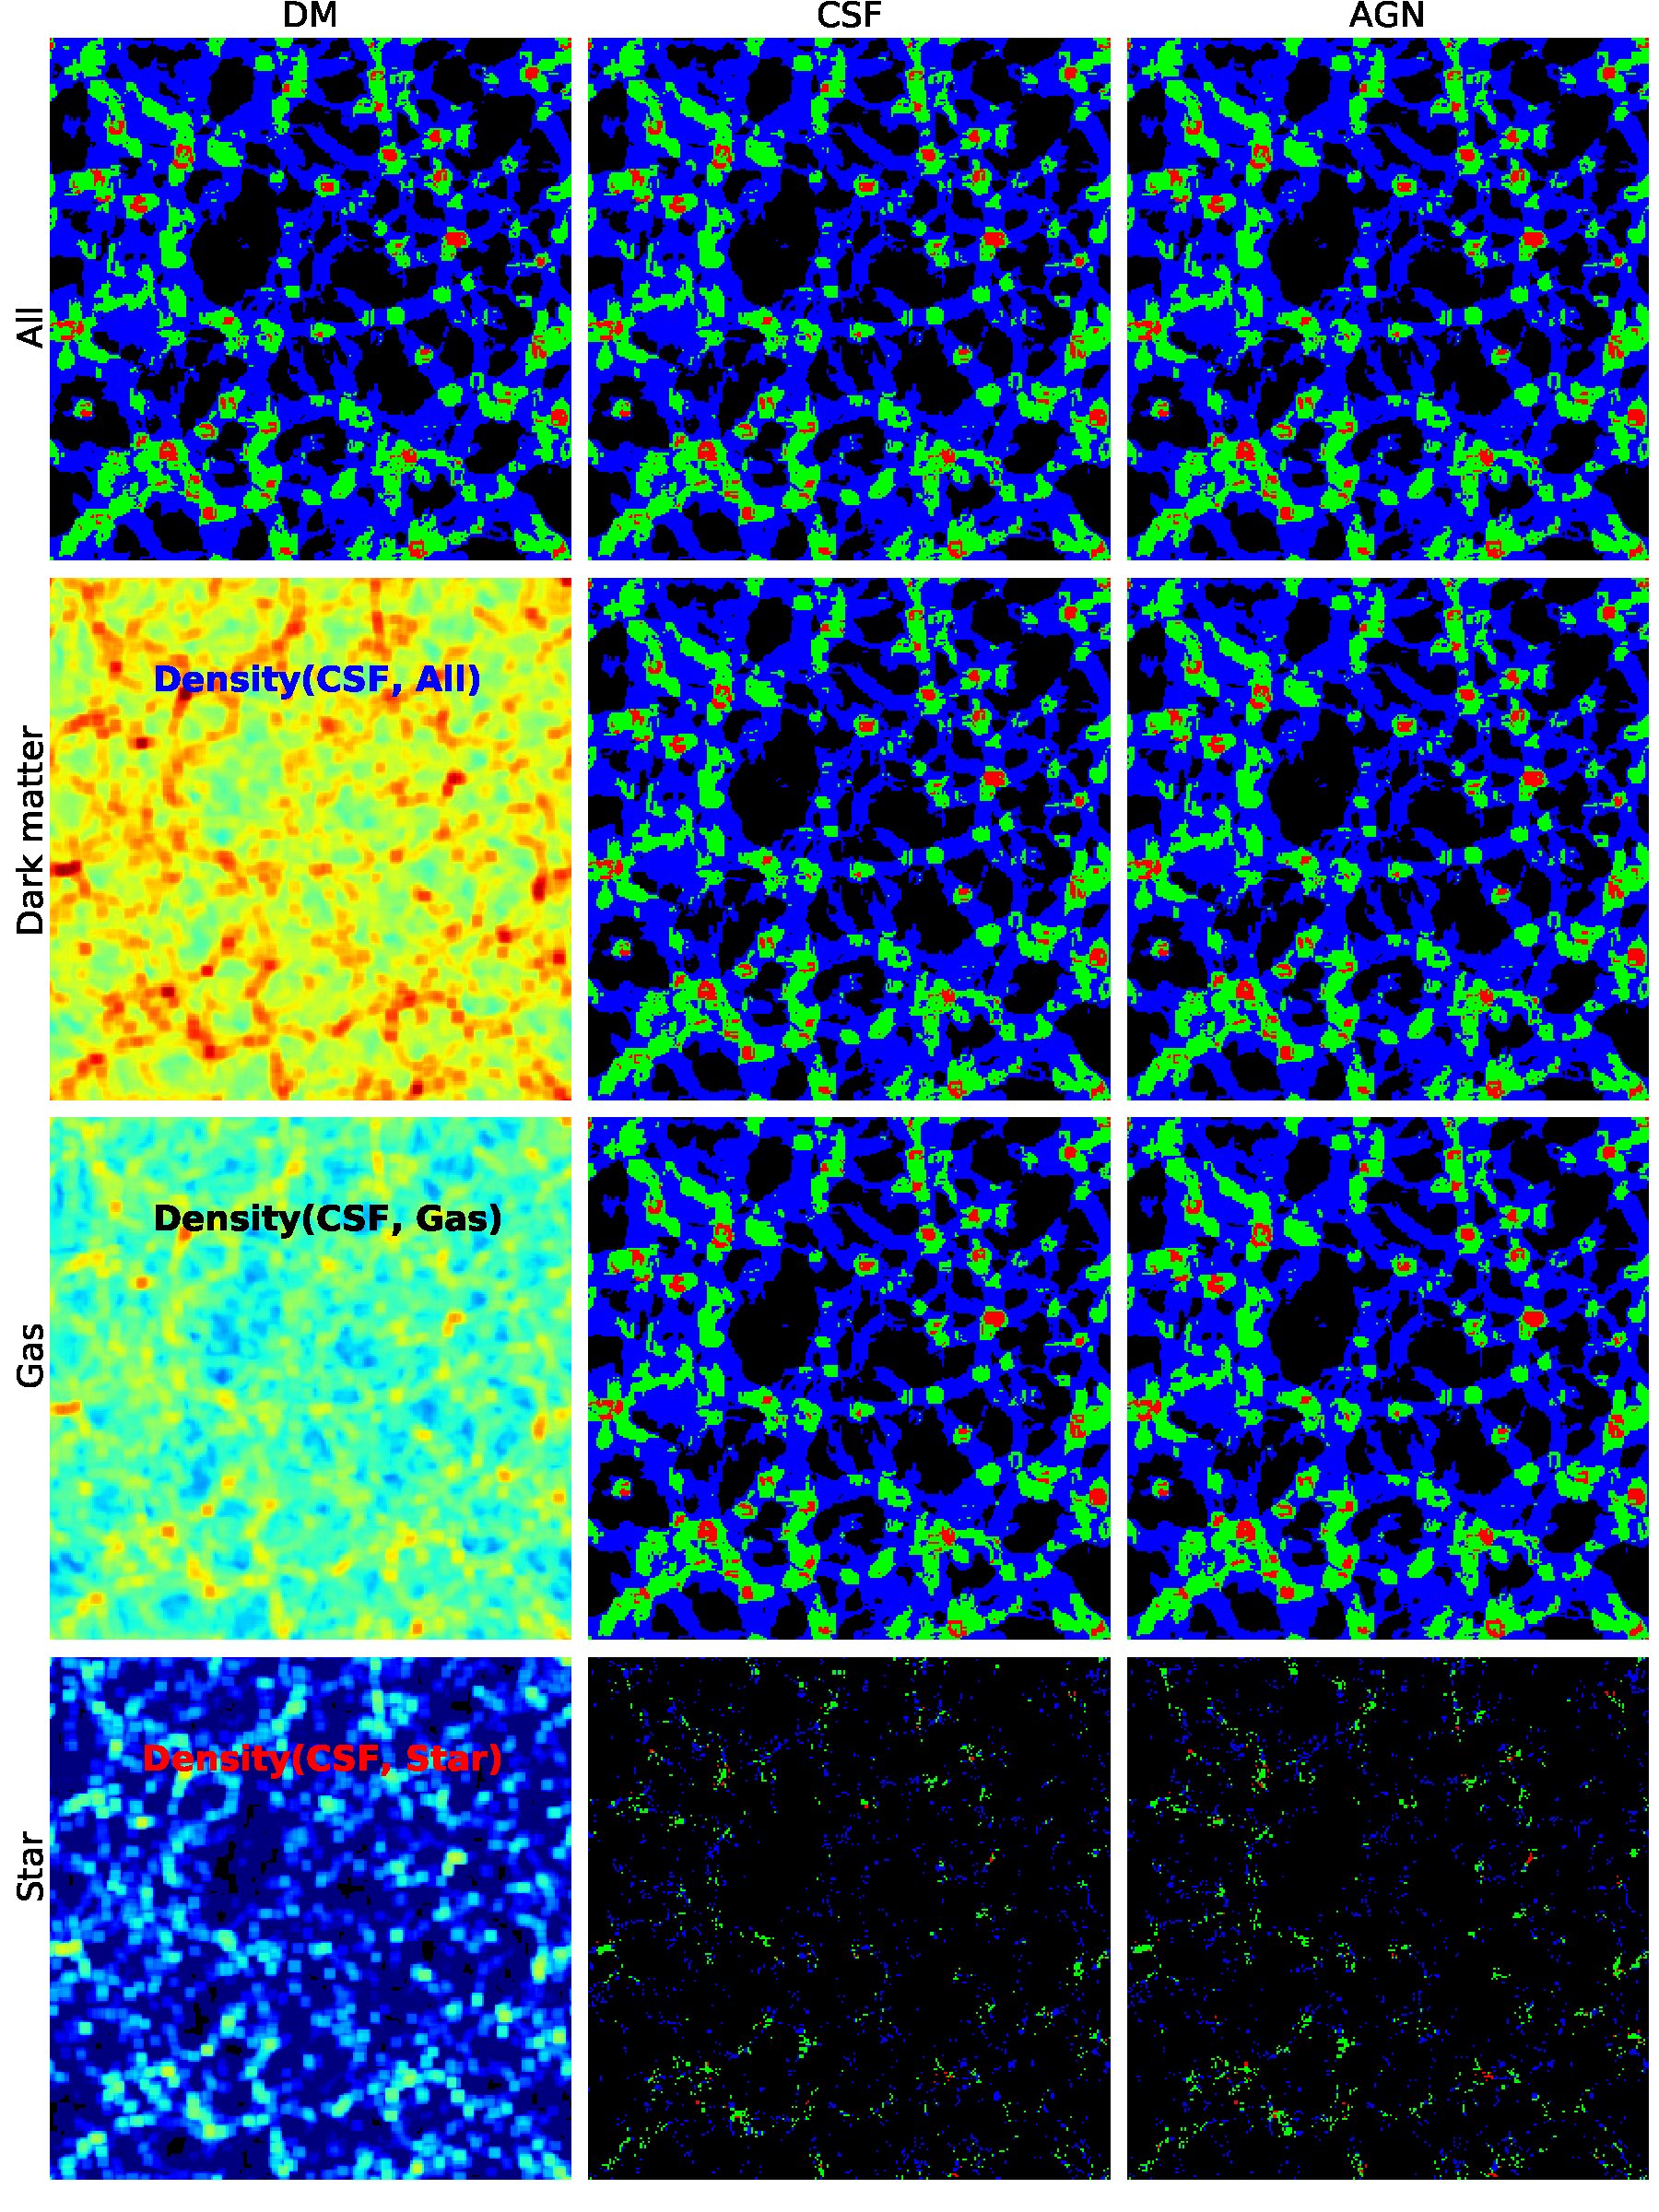
\includegraphics[height=\textheight]{image_show_V}
  \end{figure}
\end{textblock*}

\begin{textblock*}{5.5cm}(9.5cm,2cm)
{
{Illustration of the LSEs (classified with Vweb) at z = 0: black for voids, blue for sheets, green for filaments and red for knots}

\bigskip

Cui et al. 2018, LSE Paper I}
\end{textblock*}
\end{frame}

\begin{frame}{The volume and mass fractions of different large-scale structures}
\vspace{-0.3cm}
  \begin{figure}
    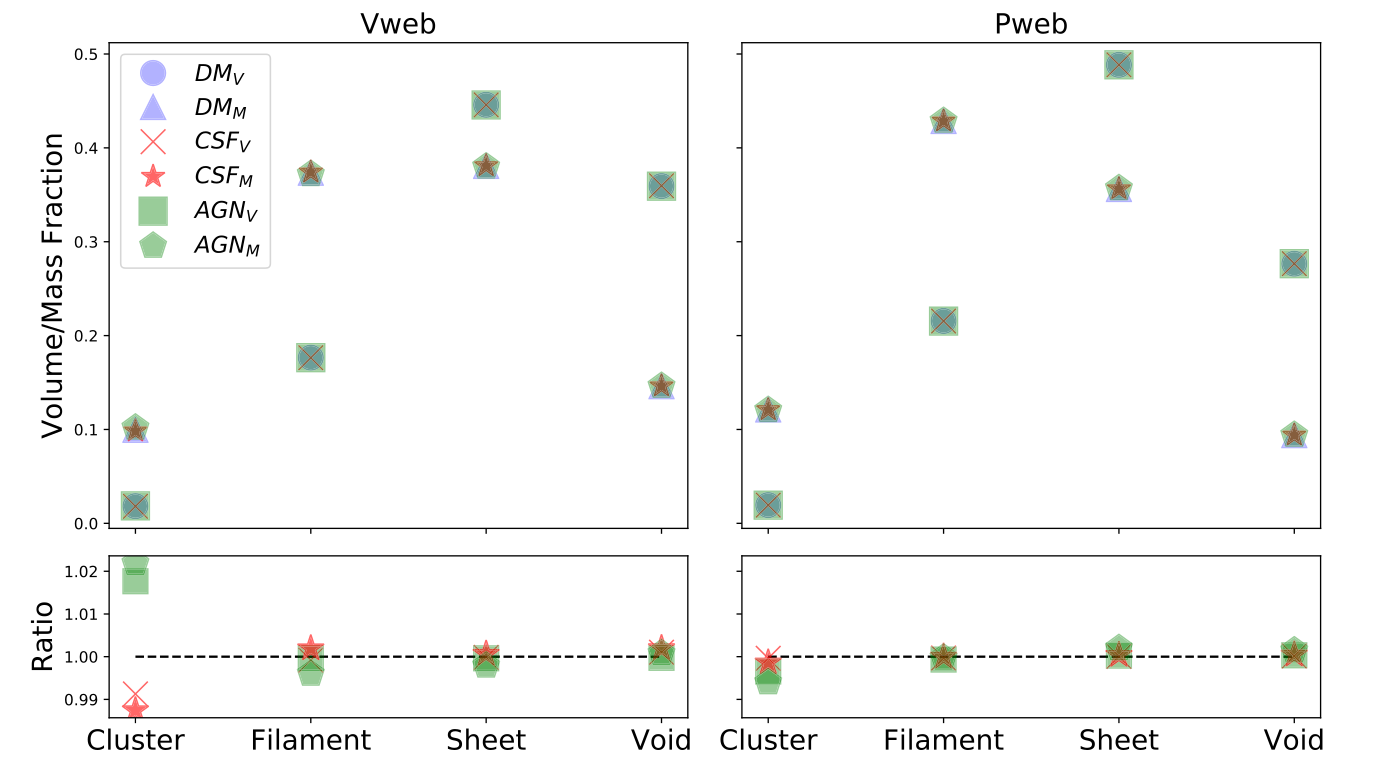
\includegraphics[height=0.85\textheight]{Fractions-BE}
  \end{figure}
\end{frame}

\begin{frame}{The consistency between gas and DM identified large-scale structures}
\vspace{-0.3cm}
  \begin{figure}
    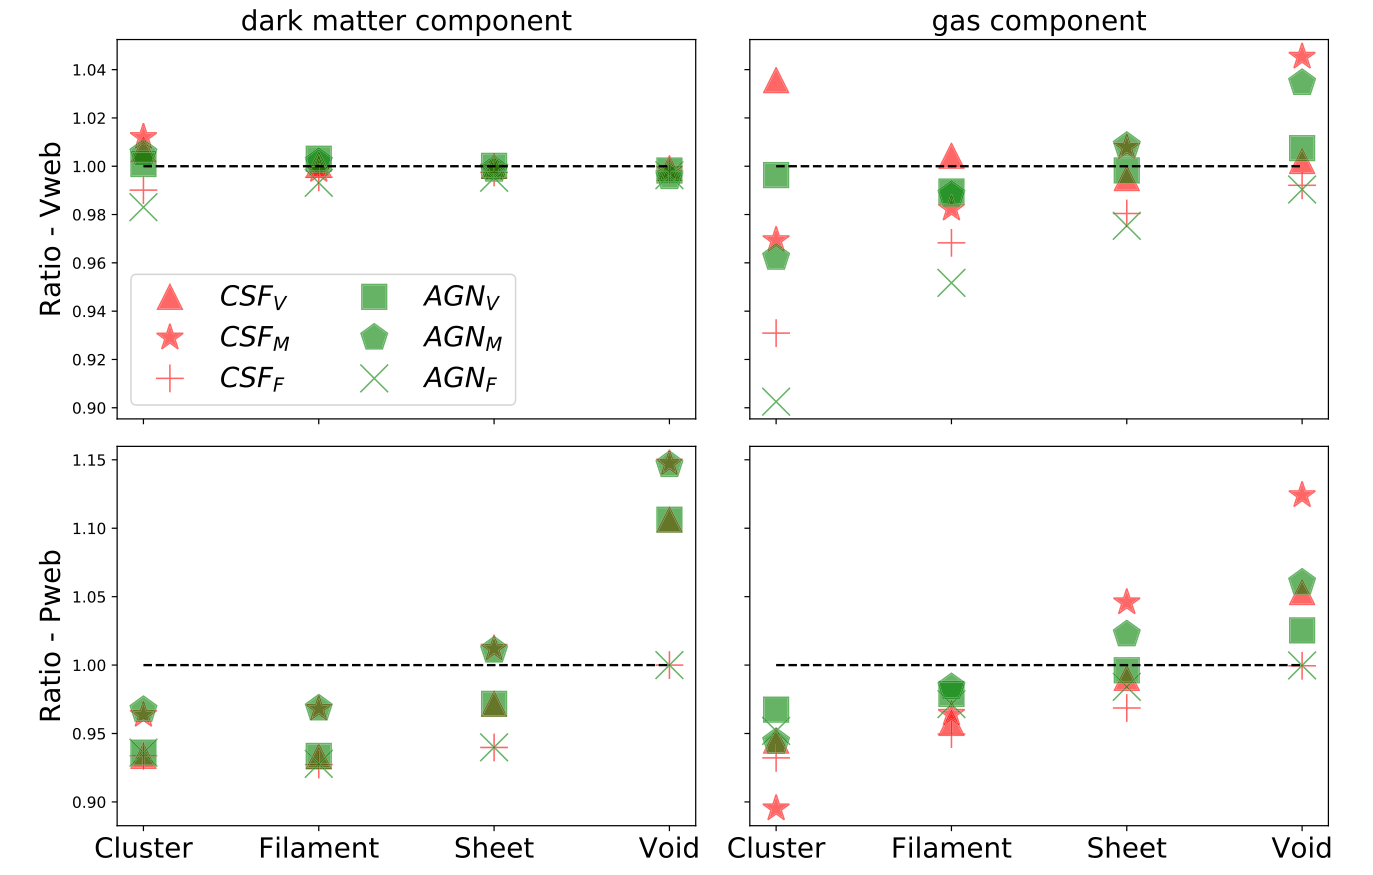
\includegraphics[height=0.85\textheight]{Fractions-gasweb}
  \end{figure}
\end{frame}

\begin{frame}[plain,c]
%   \begin{textblock*}{8cm}(3cm,4cm)
    \centering{\Huge On the evolution of the LSEs and its baryons.}
%   \end{textblock*}
\end{frame}

\begin{frame}[plain,t]
\vspace{-0.3cm}
  \begin{figure}
  \hspace{-3cm}
    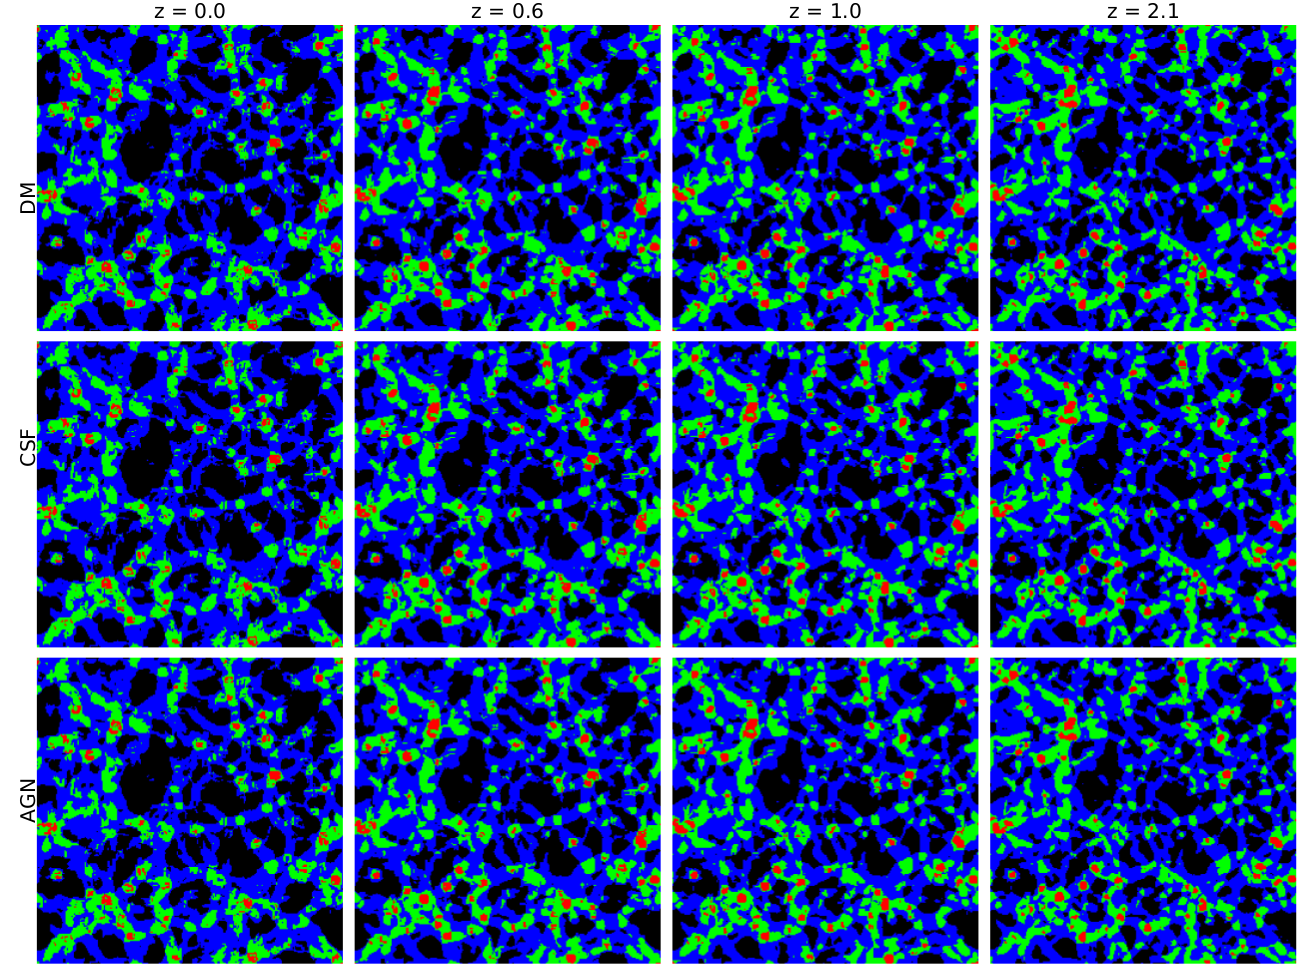
\includegraphics[height=\textheight]{Evolution-illustriation}
  \end{figure}
\begin{textblock*}{3.5cm}(12.5cm,3cm)
The redshift evolution of LSEs classified by Vweb. Cui et al. 2019
\end{textblock*}
\end{frame}

\begin{frame}{The evolution of the volume and mass fractions}
\vspace{-0.3cm}
  \begin{figure}
    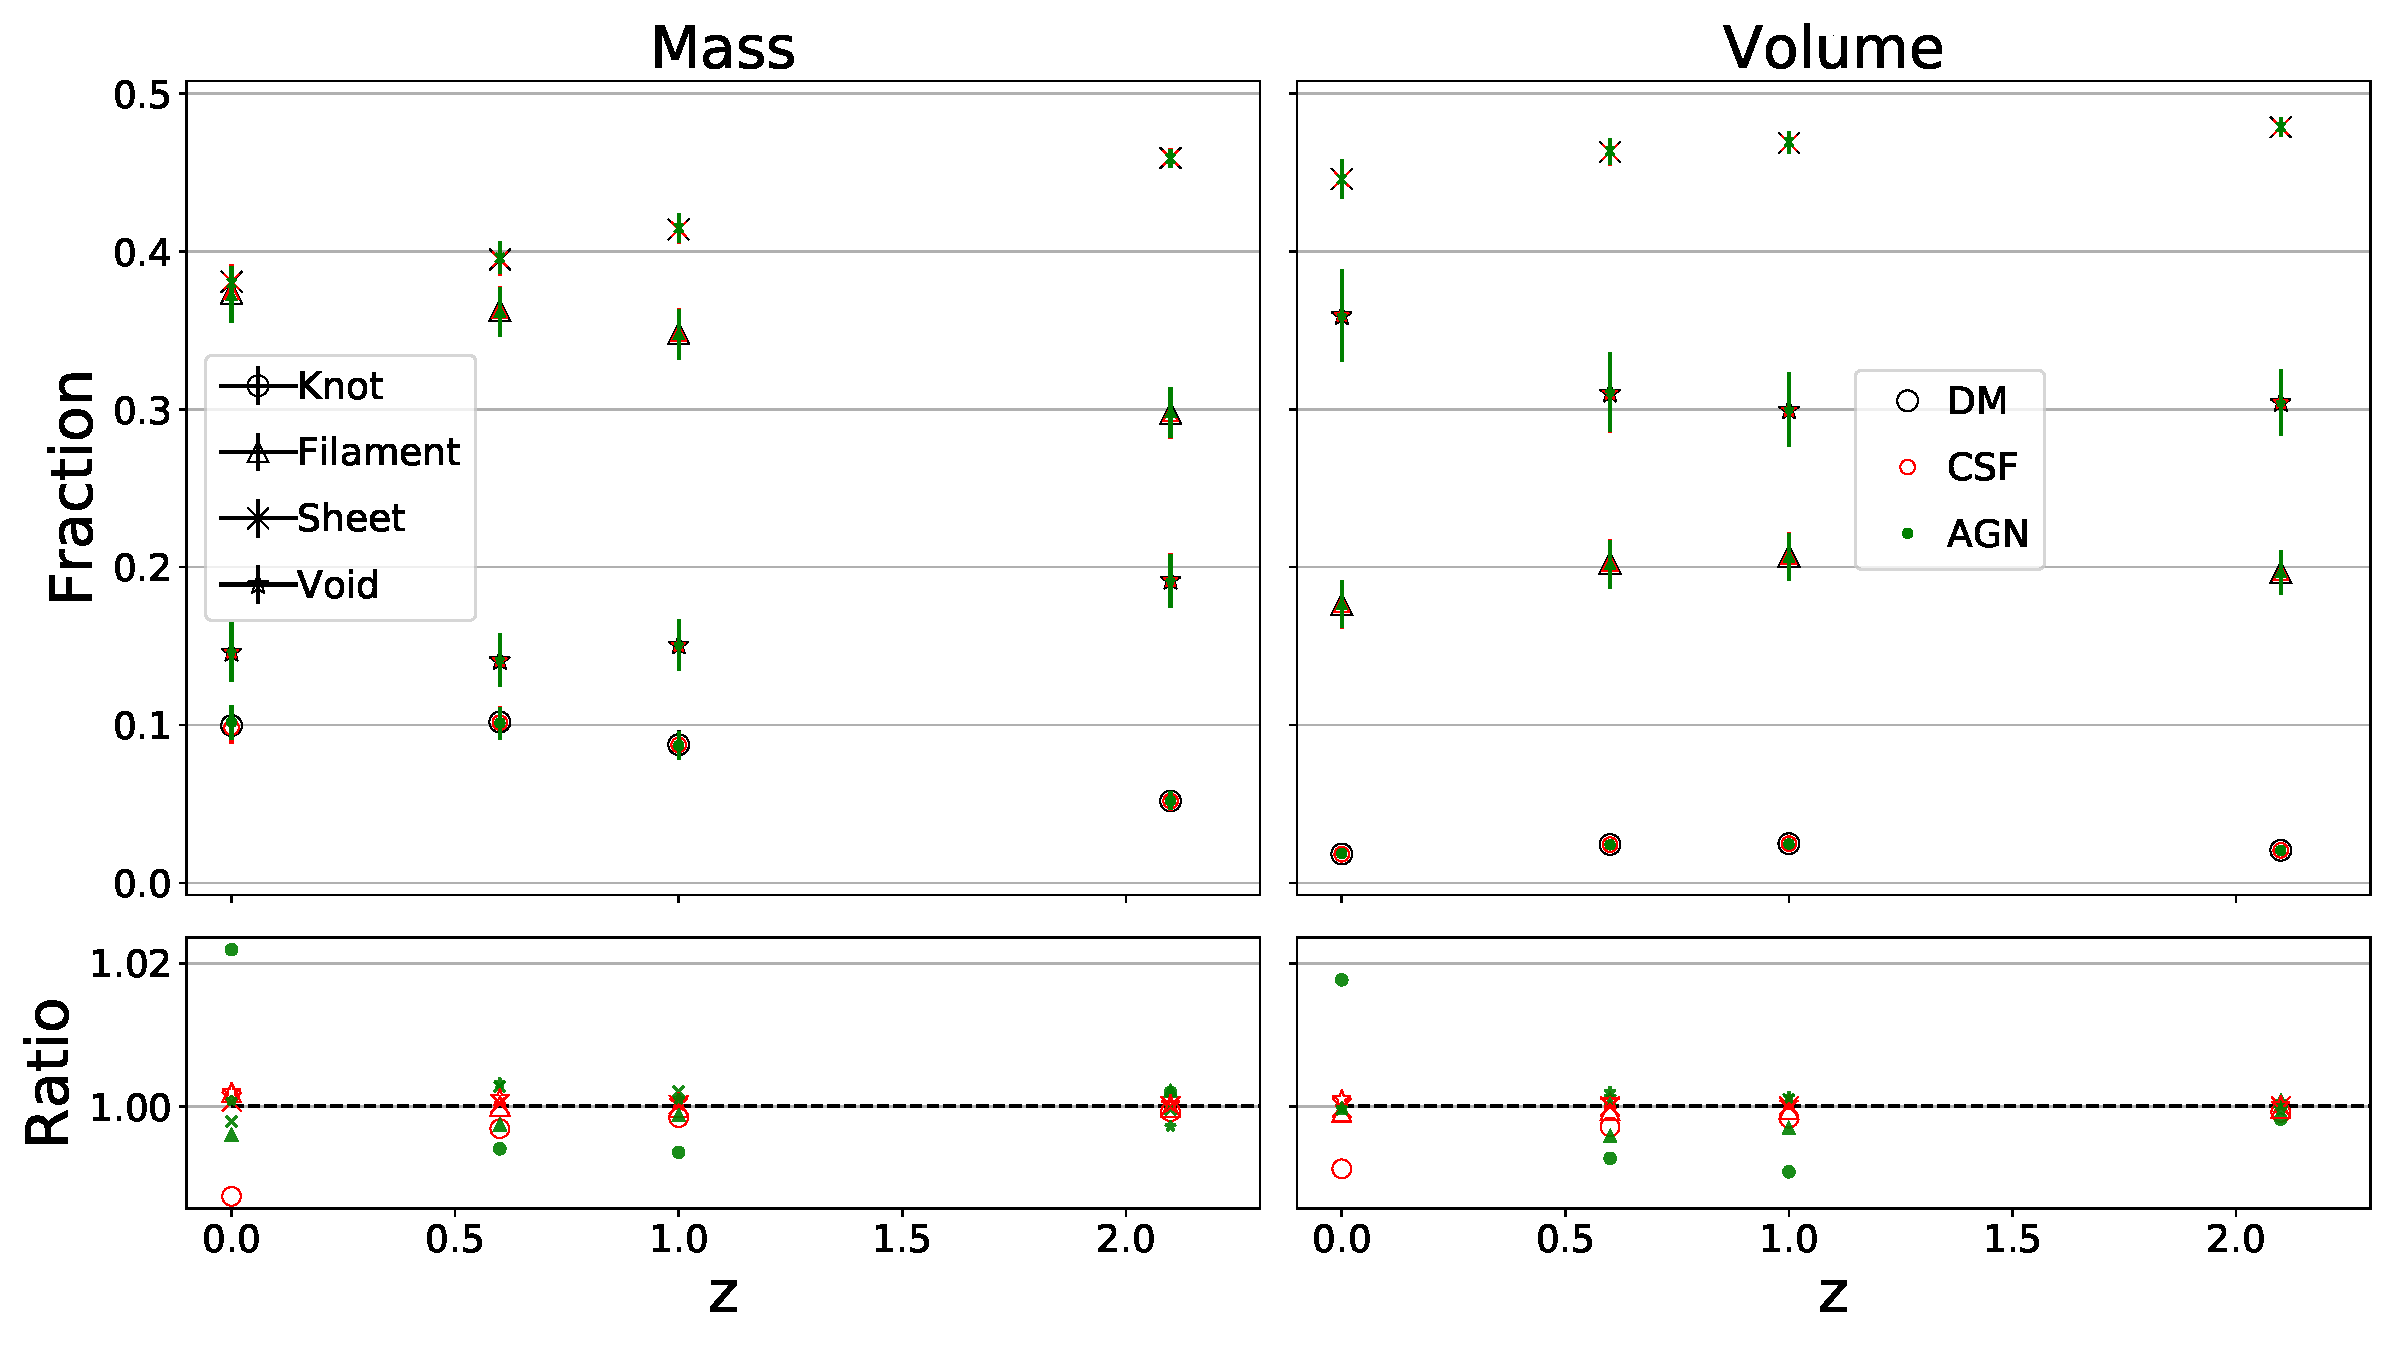
\includegraphics[height=0.9\textheight]{MV-fractions-vweb.pdf}
    \caption{The mass (left) and volume (right) fractions evolution from the Vweb method. See Zhu \& Feng, 2017 for similar results.}
  \end{figure}
\end{frame}

\begin{frame}{The consistency between baryonic and DM web}
  \begin{figure}
    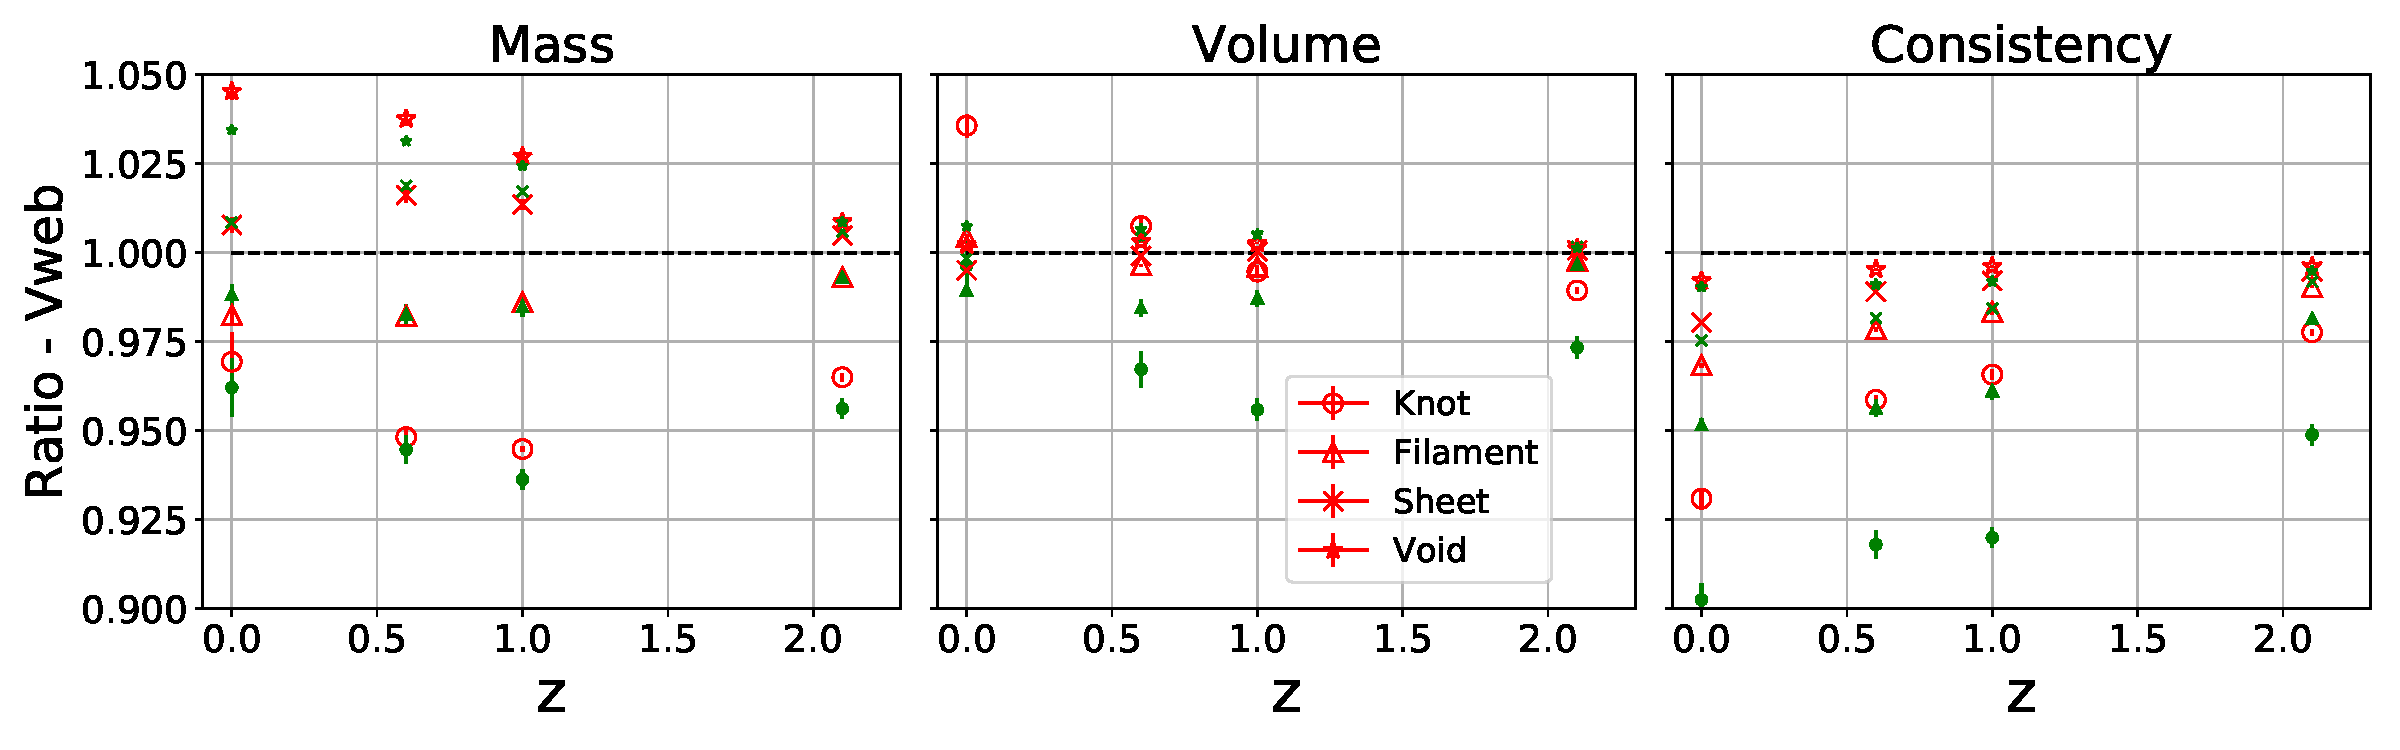
\includegraphics[width=\linewidth]{MV-fractions-diff-vweb.pdf}
    \caption{The differences between the large-scale structures classified by gas and total matter.}
  \end{figure}
\end{frame}

\begin{frame}[plain,t]
\vspace{-0.3cm}
  \begin{figure}
  \hspace{-3cm}
    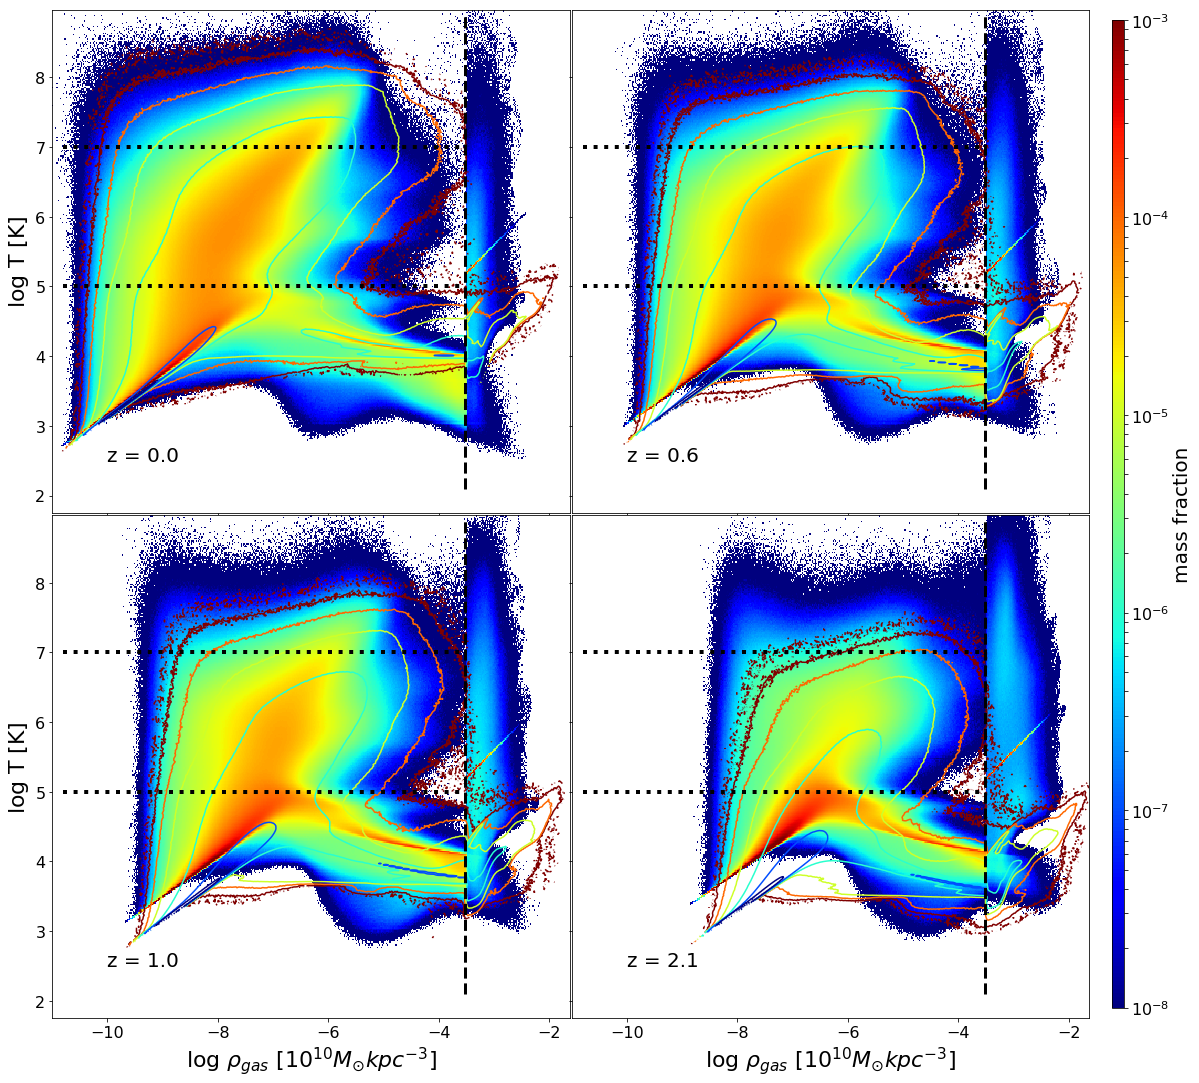
\includegraphics[height=\textheight]{RT-evolution.png}
  \end{figure}
  \begin{textblock*}{4cm}(11.5cm,3cm)
  {The evolution of the gas density-temperature diagram}
  \end{textblock*}
\end{frame}

\begin{frame}{The overall baryon fractions}
Following Dave et al. 2001, gas is separated into:
\begin{itemize}
    \item[] Hot gas: T $>$ 10$^7$ K 
    \item[] WHIM: 10$^5 >$ T $> 10^7$ K 
\end{itemize}

\begin{table}
\fontsize{8}{8}\selectfont
    \centering
    \caption{The cosmological gas and stellar mass fractions with respect to the total baryon mass.}
    \begin{threeparttable}
        \begin{tabular}{|c|c|c|c|c|}
        \hline
            Redshift & hot gas & \alert{WHIM} & cold gas & star \\
            \hline
            Nicastro et al. 2018\tnote{a} & 9$\pm$4.5 & $\gtrsim$24 \& $\lesssim$55 & 29.7$\pm$11 & 7$\pm$2\\
            Haider et al. 2016\tnote{b} & 6.5 & 53.9 & 32.8 & - \\
            z = 0   & 4.6$\pm$0.7 (4.6$\pm$0.1) & \alert{41.3}$\pm$1.1 (38.3$\pm$1.0) & 50.9$\pm$0.1 (50.6$\pm$0.2) & 3.2$\pm$0.1 (6.5$\pm$0.2)\\
            z = 0.6 & 2.4$\pm$0.4 (1.1$\pm$0.2) & \alert{34.9}$\pm$1.1 (29.7$\pm$1.1) & 60.2$\pm$0.1 (65.0$\pm$0.1) & 2.5$\pm$0.1 (4.2$\pm$0.2)\\
            z = 1.0 & 1.3$\pm$0.2 (0.3$\pm$0.0) & \alert{28.7}$\pm$1.1 (21.9$\pm$1.0) & 68.1$\pm$0.1 (74.8$\pm$0.1) & 1.9$\pm$0.1 (2.8$\pm$0.1)\\
            z = 2.1 & 0.2$\pm$0.0 (0.0$\pm$0.0) & \alert{10.8}$\pm$0.5 (6.2$\pm$0.4) & 88.2$\pm$0.1 (92.9$\pm$0.0) & 0.8$\pm$0.0 (0.8$\pm$0.0)\\
            \hline
        \end{tabular}
        \begin{tablenotes}
        \item[a] These fractions are estimated at $z<0.5$.
        \item[b] These fractions are with respect to the total gas mass at $z=0$.
        \end{tablenotes}
    \end{threeparttable}
\end{table}
\end{frame}

\begin{frame}[plain,t]
\vspace{-0.3cm}
  \begin{figure}
  \hspace{-3cm}
    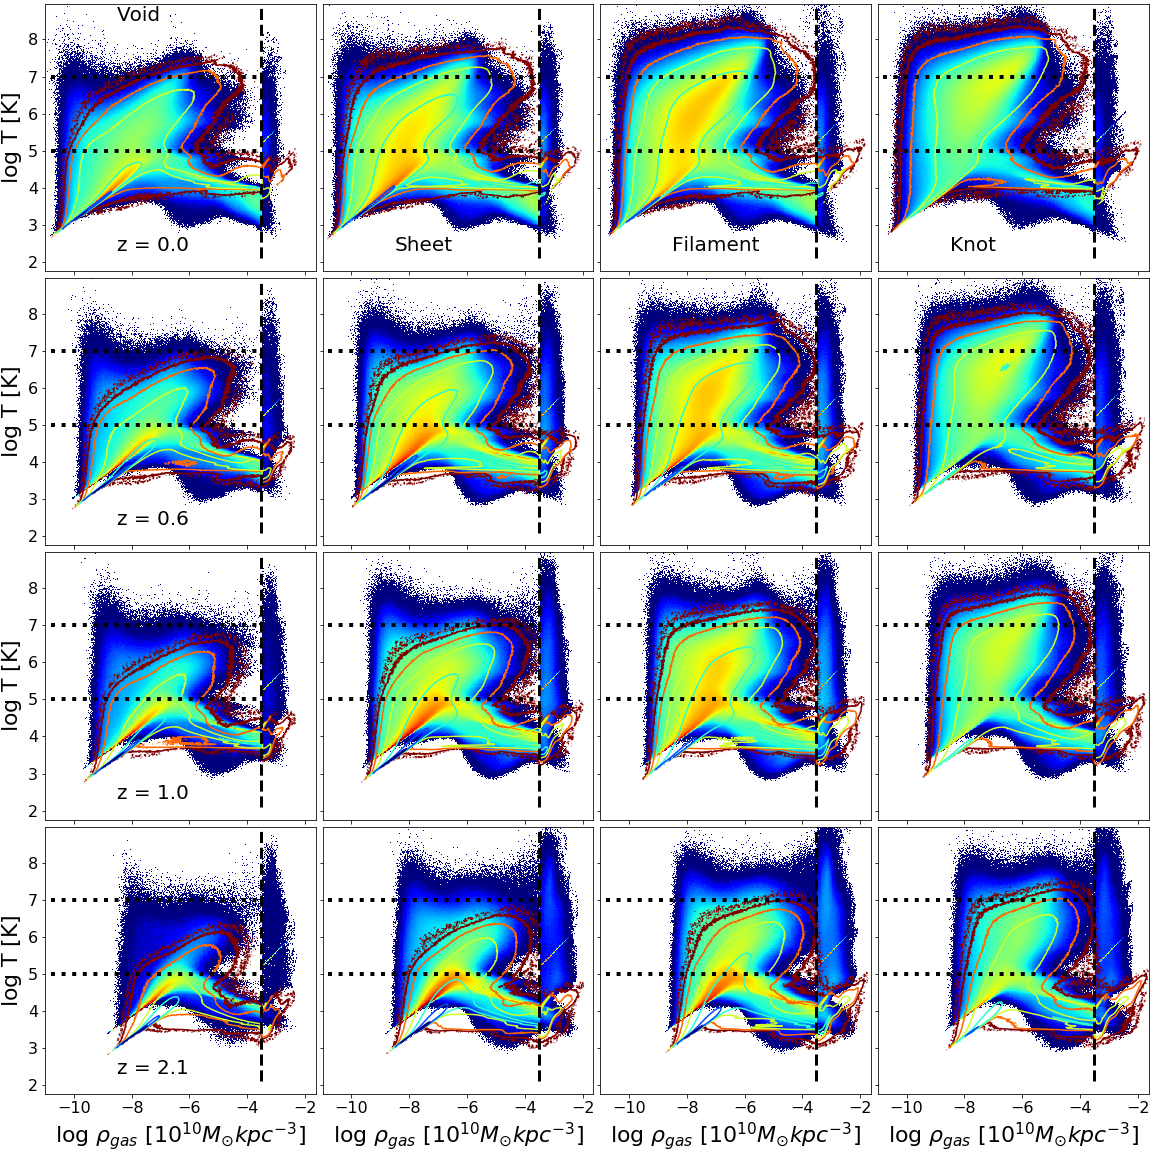
\includegraphics[height=\textheight]{RTE-evolution.png}
  \end{figure}
    \begin{textblock*}{4cm}(11.5cm,3cm)
    {The gas density-temperature diagram in different large-scale environments}
    \end{textblock*}
\end{frame}

\begin{frame}[plain,t]
\begin{table}
\fontsize{8}{8}\selectfont
\caption{The distribution of baryon components in different LSEs at the four redshifts.}
  \begin{tabular}{c|c|c|c|c}
       & Voids & Sheets & Filaments & Knots \\
       \hline
       & & z = 0 & & \\
       \hline
    $f_{\rm total\ gas}$ & 0.15$\pm$0.02 (0.16$\pm$0.02) & 0.38$\pm$0.01 (0.39$\pm$0.01) & 0.37$\pm$0.02 (0.36$\pm$0.02) & 0.10$\pm$0.01 (0.09$\pm$0.01) \\
    $f_{\rm star}$       & 0.08$\pm$0.01 (0.06$\pm$0.01) & 0.33$\pm$0.02 (0.29$\pm$0.02) & 0.44$\pm$0.01 (0.48$\pm$0.01) & 0.15$\pm$0.02 (0.17$\pm$0.02) \\
    $f_{\rm hot\ gas}$   & 0.00$\pm$0.00 (0.00$\pm$0.00) & 0.04$\pm$0.01 (0.05$\pm$0.01) & 0.46$\pm$0.03 (0.50$\pm$0.03) & 0.49$\pm$0.03 (0.45$\pm$0.03) \\
    \alert{$f_{\rm WHIM}$}      & 0.05$\pm$0.01 (0.06$\pm$0.01) & 0.30$\pm$0.02 (0.31$\pm$0.02) & \alert{0.51}$\pm$0.01 (0.50$\pm$0.01) & 0.14$\pm$0.01 (0.13$\pm$0.01) \\
    $f_{\rm cold\ gas}$  & 0.25$\pm$0.02 (0.25$\pm$0.02) & 0.48$\pm$0.01 (0.48$\pm$0.01) & 0.24$\pm$0.02 (0.25$\pm$0.02) & 0.03$\pm$0.01 (0.03$\pm$0.01) \\
    \hline
       & & z = 0.6 & & \\
       \hline
    $f_{\rm total\ gas}$ & 0.14$\pm$0.02 (0.14$\pm$0.02) & 0.39$\pm$0.01 (0.39$\pm$0.01) & 0.37$\pm$0.02 (0.36$\pm$0.02) & 0.11$\pm$0.01 (0.11$\pm$0.01) \\
    $f_{\rm star}$       & 0.05$\pm$0.01 (0.03$\pm$0.00) & 0.28$\pm$0.02 (0.22$\pm$0.02) & 0.47$\pm$0.01 (0.48$\pm$0.01) & 0.21$\pm$0.02 (0.27$\pm$0.02) \\
    $f_{\rm hot\ gas}$   & 0.00$\pm$0.00 (0.00$\pm$0.00) & 0.01$\pm$0.00 (0.00$\pm$0.00) & 0.23$\pm$0.01 (0.15$\pm$0.02) & 0.76$\pm$0.02 (0.85$\pm$0.02) \\
    \alert{$f_{\rm WHIM}$}       & 0.03$\pm$0.00 (0.03$\pm$0.00) & 0.25$\pm$0.02 (0.23$\pm$0.02) & \alert{0.53}$\pm$0.01 (0.52$\pm$0.01) & 0.20$\pm$0.01 (0.22$\pm$0.01) \\ 
    $f_{\rm cold\ gas}$  & 0.21$\pm$0.02 (0.19$\pm$0.02) & 0.48$\pm$0.01 (0.47$\pm$0.01) & 0.28$\pm$0.02 (0.29$\pm$0.02) & 0.04$\pm$0.01 (0.04$\pm$0.01) \\
    \hline
      & & z = 1.0 & & \\
      \hline
    $f_{\rm total\ gas}$ & 0.14$\pm$0.02 (0.14$\pm$0.02) & 0.40$\pm$0.01 (0.40$\pm$0.01) & 0.36$\pm$0.02 (0.35$\pm$0.02) & 0.10$\pm$0.01 (0.10$\pm$0.01) \\
    $f_{\rm star}$       & 0.03$\pm$0.01 (0.02$\pm$0.00) & 0.26$\pm$0.02 (0.20$\pm$0.02) & 0.48$\pm$0.01 (0.48$\pm$0.01) & 0.22$\pm$0.02 (0.29$\pm$0.02) \\
    $f_{\rm hot\ gas}$   & 0.00$\pm$0.00 (0.00$\pm$0.00) & 0.02$\pm$0.01 (0.00$\pm$0.00) & 0.22$\pm$0.02 (0.08$\pm$0.02) & 0.76$\pm$0.02 (0.91$\pm$0.02)\\
    \alert{$f_{\rm WHIM}$}       & 0.02$\pm$0.00 (0.02$\pm$0.00) & 0.24$\pm$0.01 (0.21$\pm$0.01) & \alert{0.53}$\pm$0.01 (0.52$\pm$0.01) & 0.21$\pm$0.01 (0.25$\pm$0.01) \\
    $f_{\rm cold\ gas}$  & 0.20$\pm$0.02 (0.18$\pm$0.02) & 0.48$\pm$0.01 (0.46$\pm$0.01) & 0.28$\pm$0.02 (0.31$\pm$0.02) & 0.04$\pm$0.01 (0.05$\pm$0.01) \\
    \hline
      & & z = 2.1 & & \\
      \hline
    $f_{\rm total\ gas}$ & 0.18$\pm$0.02 (0.18$\pm$0.02) & 0.45$\pm$0.01 (0.45$\pm$0.01) & 0.31$\pm$0.02 (0.31$\pm$0.02) & 0.06$\pm$0.01 (0.06$\pm$0.01) \\
    $f_{\rm star}$       & 0.02$\pm$0.00 (0.02$\pm$0.00) & 0.23$\pm$0.02 (0.20$\pm$0.01) & 0.52$\pm$0.01 (0.50$\pm$0.01) & 0.24$\pm$0.02 (0.28$\pm$0.02) \\
    $f_{\rm hot\ gas}$   & 0.00$\pm$0.00 (0.00$\pm$0.00) & 0.07$\pm$0.01 (0.00$\pm$0.00) & 0.35$\pm$0.02 (0.04$\pm$0.03) & 0.58$\pm$0.03 (0.96$\pm$0.03) \\
    \alert{$f_{\rm WHIM}$}      & 0.02$\pm$0.00 (0.01$\pm$0.00) & 0.24$\pm$0.01 (0.18$\pm$0.01) & \alert{0.58}$\pm$0.01 (0.53$\pm$0.01) & 0.23$\pm$0.01 (0.28$\pm$0.02) \\
    $f_{\rm cold\ gas}$  & 0.20$\pm$0.02 (0.19$\pm$0.02) & 0.47$\pm$0.01 (0.47$\pm$0.01) & 0.28$\pm$0.02 (0.30$\pm$0.02) & 0.04$\pm$0.01 (0.05$\pm$0.01) \\
    \hline
  \end{tabular}
\end{table}
\end{frame}

\section{conclusion and future prospects}
\begin{frame}
  \frametitle{Conclusion}
  {\Large
  \begin{itemize}
    \item The baryon models have a weak impact on the matter distributions at large scale.
    \item Gas is a unbiased tracer of dark matter for these large-scale structures, especially filament.
    \item Although the whole gas is almost equally assigned into sheet and filaments, the most WHIM is located in the filament structures while the cold gas is basically located in sheets.
  \end{itemize}}
\end{frame}

\begin{frame}[plain,c]
  \begin{center}
      {\huge Future prospects: \\ How can we observe the WHIM?}
      
      Build mock observation images (soft X-ray band) with different emission lines (O VII, etc.) and connect to the theoretical predicted WHIM abundance in order to use the next generation X-ray telescopes, such Athena\footnote{https://www.the-athena-x-ray-observatory.eu/}, HUBS\footnote{http://hubs.phys.tsinghua.edu.cn/en/index.html}, to detect WHIM.
      
      \bigskip
      
      \bigskip
      
      {\huge How can we observe the cold gas?}
      
      Build mock radio maps and understand their distribution with the next generation radio telescopes, such as SKA\footnote{https://www.skatelescope.org/}.
  \end{center}
%   \frametitle{Future prospects}
%   Connecting hydrodynamical simulations with observations through mock images.
%   \begin{itemize}
%     \item Optical: pymgal
%     \item Xray: pymxc 
    
%         spectrum is coming from Xspec library, interpolated with gas properties from hydrosimulations to produce the SIMPUT format, this file will use SIXTE (a monte-carlo simulation toolkit for the Athen XIFU) to produce the eventlist.
%     \item SZ: pymsz
%     \item Radio: pymr
%   \end{itemize}

%   \only<2>{
%   My personal interests to HUBS:
%   \begin{itemize}
%     \item[1] theoretical analysis pipeline with pymxc.
%     \item[2] Using HUBS to constrain cosmology models/parameters.
%   \end{itemize}}
\end{frame}

\begin{frame}[plain, c]
    \begin{center}
        \Huge{Thank you}

    \bigskip
    
    \bigskip
    
    \bigskip
    
    {\small \bf Acknowledgements:}
    
    
\includegraphics[height=1cm]{ifalogo.jpg}
    
\includegraphics[height=1cm]{cosform_logo.png}
    
\includegraphics[height=1cm]{logo_uam.jpg}
    \end{center}
\end{frame}

\end{document}
